When we consider Poncelet 3-periodic families, a natural (and indeed early) question was ``what are the loci of certain traingle centers''. Recall one of our early experimental finds: that over billiard 3-periodics, the locus of the incenter $X_1$ is an ellipse (as is that of the excenters), see \cref{sec:02-inc-exc-loci}. Also an early find was that the ``locus'' of the Mittenpunkt $X_9$ is a point, see \cref{sec:02-stationary}.

In this chapter we expand on this exploration of loci of triangle centers, touring a gallery of interesting locus-related phenomena, including:

\begin{itemize}
    \item The loci of some notable centers of a triangle, showing thy are ellipses;
    \item Billiard 3-periodics which can be both acute and obtuse;
    \item A triangle center with a non-elliptic (quartic) locus nearly identical to an ellipse;
    \item Two special triangle centers railed to either the billiard or the confocal caustic;
    \item A non-smooth locus with four singularities;
    \item A self-intersecting locus;
    \item A non-compact, non-elliptic locus;
    \item An elliptic locus whose aspect ratio is the golden ratio $\varphi$;
    \item A triangle center railed to the elliptic billiard whose motion with respect to 3-periodic vertices is ``non-monotonic'';
    \item The non-elliptic loci of the vertices of certain derived triangles. 
    \item The ``triple-winding'' of triangle center loci over themselves.
\end{itemize}

\section{Kimberling centers with elliptic loci}

The semi-axes $a_1,b_1$ for the elliptic locus of the incenter $X_1$ were given in \cref{thm:02-incenter-excenter}. It turns the loci of the next four centers in \cite{etc} are also ellipses. There are the barycenter $X_2$, the circumcenter $X_3$, the orthocenter $X_4$, and the center of the 9-point circle (also known as Euler's circle) $X_5$. Their semi-axes are given by:

\begin{align*}
    \left(a_2,b_2\right)=&k_2\left(a,b\right),\;\text{with}\; k_2=\frac{2\delta -a^{2}-b^{2}}{3c^2}\\
     \left(a_3,b_3\right)=&\left(\frac{a^{2}-\delta}{2a},\frac{\delta-b^{2}}{2b}\right)\\
 \left(a_4,b_4\right)=&\left(\frac{k_4}a,\frac{k_4}b\right),\;\text{with}\;k_4=\frac{  (a^{2}+b^{2})\delta-2\,a^{2}b^{2} }{c^2}\\
   \left(a_5,b_5\right)=&\left(\frac{- w'_5(a,b)+ w''_5(a,b) \delta}{ w_5(a,b)},\;\frac{ w'_5(b,a)-{w''_5(b,a) \delta}}{w_5(b,a)}\right)
\end{align*}
where $w'_5(u,v)=u^2(u^2+3v^2)$, $w''_5(u,v)=3u^2+ v^2$, and $w_5(u,v)=4u(u^2-v^2)$. Note that (i) $a_2/b_2=a/b$ and (ii) $b_4/a_4=a/b$.

As it turns out, the locus of 49 out of the first 200 centers in \cite{etc} are ellipses. These are: $X_k$, $k=$1,  2,  3,  4,  5,  7,  8,  10,  11,  12,  20,  21,  35,  36,  40,  46,  55,  56,  57,  63,  65,  72,  78,  79,  80,  84,  88,  90,  100,  104,  119,  140,  142,  144,  145,  149,  153,  162,  165,  190,  191,  200. Links to live animations as well as expressions for their semi-axes are provided in \cite{garcia2021-ellipses-web}.

%% Swans
%% the following centers lie on the $X_9$-centered circumellipse: 88, 100, 162, 190 \cite{etc}.

\begin{figure}
\centering
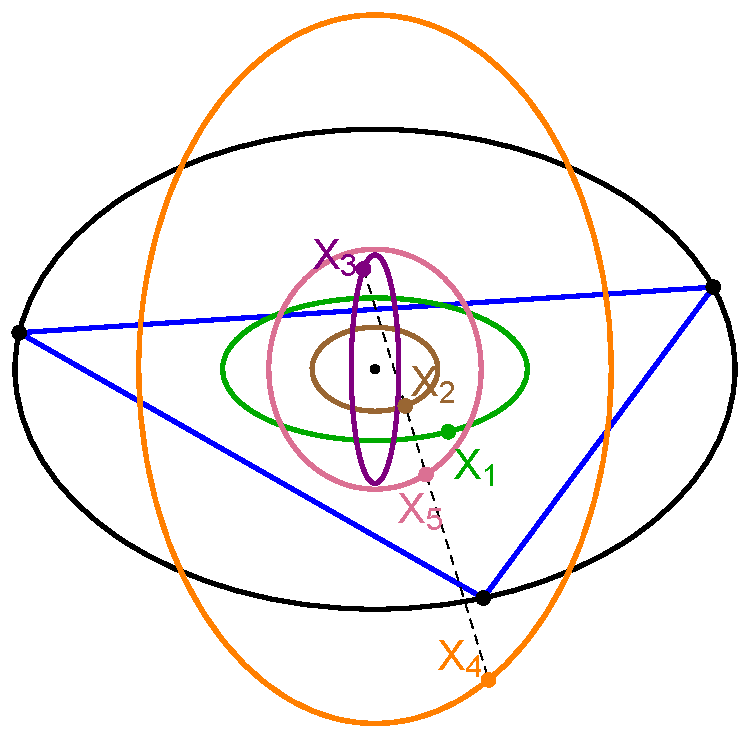
\includegraphics[width=.6\textwidth]{pics_05_060_locus_x12345.pdf}
\caption{Over billiard 3-periodics, the loci of incenter $X_1$, barycenter $X_2$, circumcenter $X_3$, orthocenter $X_4$, and 9-point center $X_5$ are all ellipses. The Euler line (dashed black) is shown passing through all but the first center. \href{https://youtu.be/sMcNzcYaqtg}{Video}, \href{https://bit.ly/3eVScgE}{Live}}
\label{fig:05-x12345}
\end{figure}

%%% begin X4
\section{When billiard 3-periodics are obtuse}

\begin{figure}
    \centering
    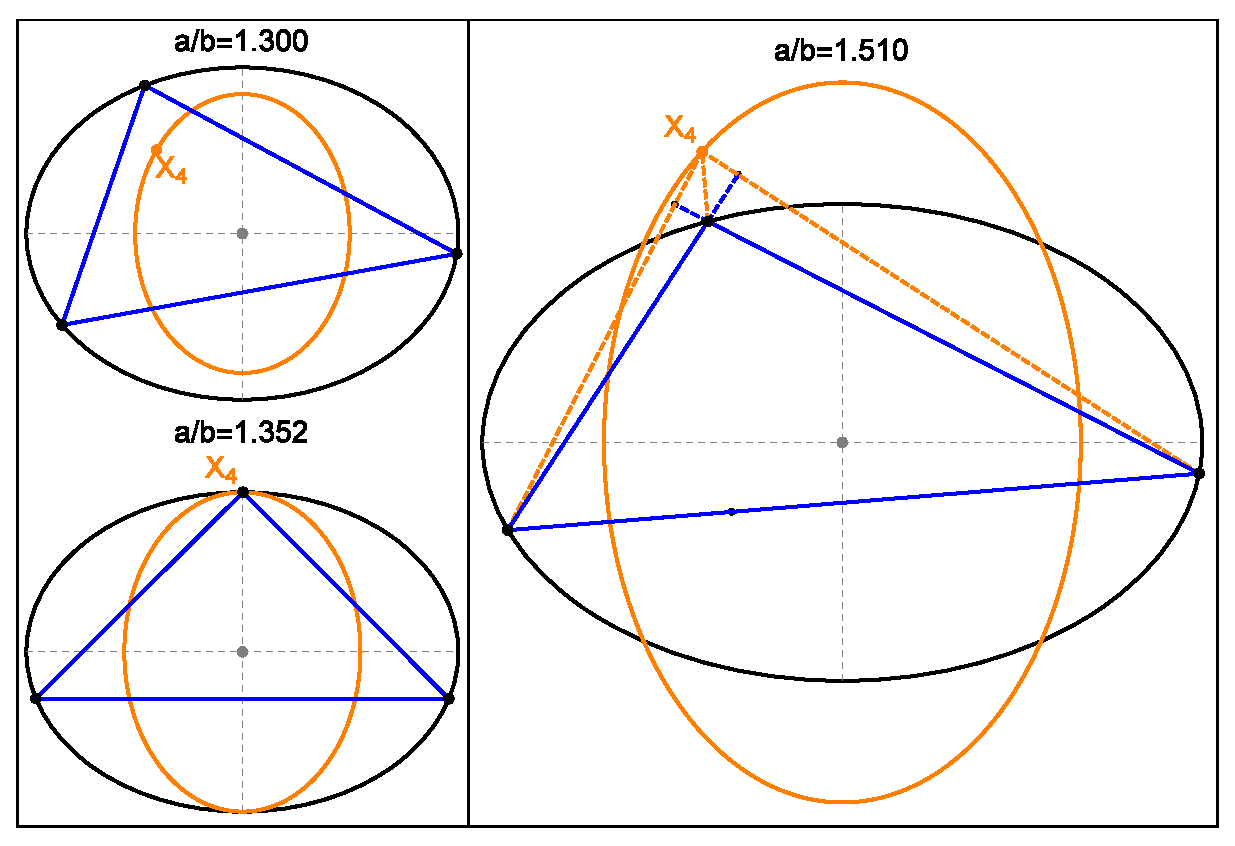
\includegraphics[width=\textwidth]{pics_05_130_ort_loci}
    \caption{Locus of the orthocenter (orange) over elliptic billiards with different aspect ratios. If $a/b$ is (i) less than (resp. (ii) equal, (iii) greater than) $\alpha_4{\simeq}1.352$, the locus of the orthocenter $X_4$ (orange) is (i) interior (resp. (ii) internally tangent, (iii) intersecting) with the elliptic billiard. In (i) and (ii) all 3-periodics are acute, whereas in (iii) some will be obtuse.}
    \label{fig:05-orthocenter-loci}
\end{figure}

It turns out the locus of $X_4$ can be used to determine if the billiard 3-period family will contain obtuse triangles. Referring to Figure~\ref{fig:05-orthocenter-loci}:

\begin{proposition}
The locus of $X_4$ is internally tangent to the elliptic billiard at its top and bottom vertices when $a/b=\alpha_4$ given by:

\[\alpha_4 = \sqrt{2\,\sqrt {2}-1}\;{\simeq}\;1.352.\]
\label{prop:05-alpha4}
\end{proposition}

\begin{proof}
The equation $b_4=b$ is equivalent to $a^4+2a^2b^2-7b^4=0.$ Therefore, as $a>b>0$, it follows that $a/b=\sqrt{2\,\sqrt {2}-1}.$
\end{proof}

\noindent Let $\alpha_4^*$ be the positive root of
${x}^{6}+{x}^{4}-4\,{x}^{3}-{x}^{2}-1=0$, i.e.,
$\alpha_4^{*}={\simeq}\;1.51$. 

\begin{proposition}
When $a/b=\alpha_4^{*}$, then $a_4=b$ and $b_4=a$, i.e., the locus of $X_4$ is identical to a rotated copy of Billiard. 
\end{proposition}

\begin{proof}
The condition $a_4=b$, or equivalently $b_4=a$, is defined by $a^6+a^4b^2-4a^3b^3-a^2b^4-b^6=0$. Graphic analysis shows that ${x}^{6}+{x}^{4}-4\,{x}^{3}-{x}^{2}-1=0$ has only one positive real root which we call $\alpha_4^*$.
\end{proof}

\begin{theorem}
If $a/b<\alpha_4$ (resp. $a/b>\alpha_4$) the 3-periodic family will not (resp. will) contain obtuse triangles.
\end{theorem}

\begin{proof}
If the 3-periodic is acute, $X_4$ is in its interior, therefore also internal to the EB. If the 3-periodic is a right triangle, $X_4$ lies on the right-angle vertex and is therefore on the EB. If the 3-periodic is obtuse, $X_4$ lies on exterior wedge between sides incident on the obtuse vertex (feet of altitudes are exterior). Since the latter is on the EB, $X_4$ is exterior to the EB.
\end{proof}

Another way to think of this is depicted in \cref{fig:05-obtuse-zones}: $a/b>\alpha_4$, opens up two ``zones'' along the top and bottom halves of the elliptic billiard. A 3-periodic will be obtuse if and only if one of its vertices is on either zone. These zones are precisely portions of the elliptic billiard which are interior to the locus of $X_4$; see \cref{fig:05-orthocenter-loci}(right). When $a/b=\alpha_4$ said zones collapse to the top and bottom vertices of the elliptic billiard; see \cref{fig:05-orthocenter-loci}(bottom left).

\begin{figure}
    \centering
    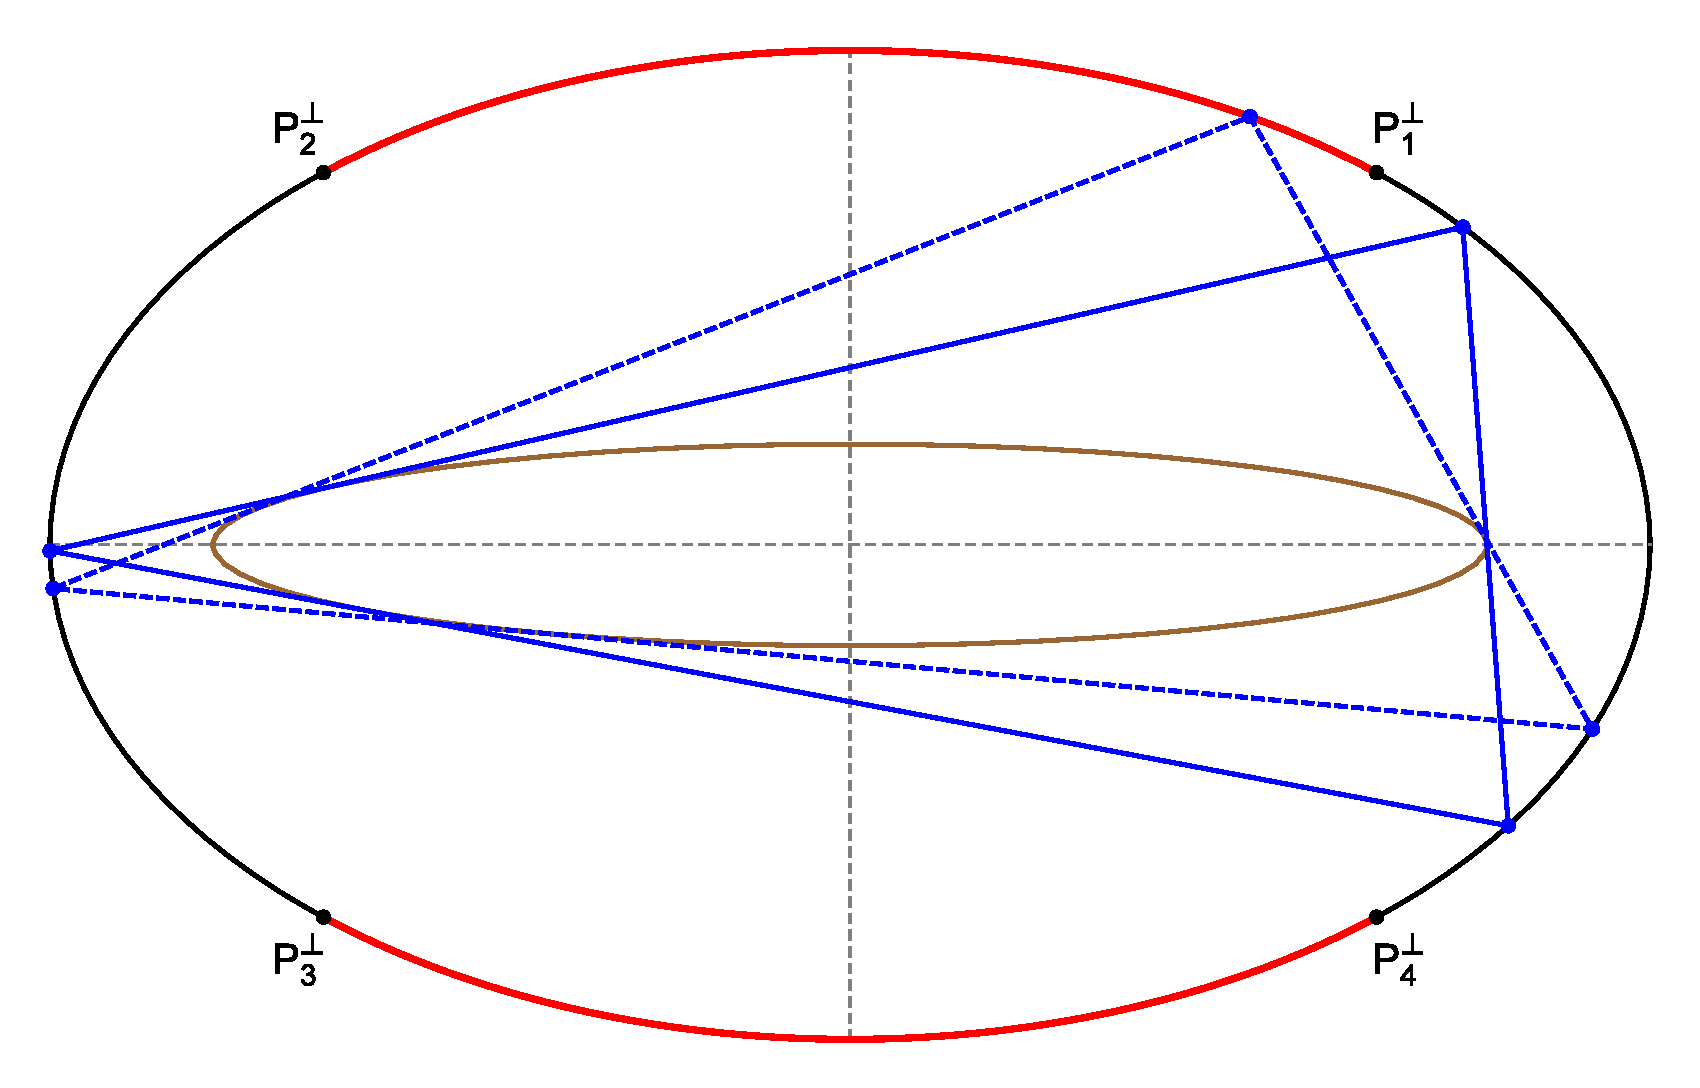
\includegraphics[width=.66\textwidth]{pics_05_150_rect_zones}
    \caption{Both acute (blue) and obtuse (dashed blue) billiard 3-periodics are shown. In this case $a/b=1.618>\alpha_4$. If a 3-periodic vertex is located in the red arcs along the top and bottom halves of the elliptic billiard, the 3-periodic will be obtuse.}
\label{fig:05-obtuse-zones}
\end{figure}

%%% end X4

%%% begin X6
\section{Quartic locus of the symmedian point \torp{$X_6$}{X(6)}}
\label{sec:symmedian}

The symmedian point $X_6$ is replete with properties, indeed it is known as the crown jewel of triangle geometry \cite[Symmedian Point]{mw}. Its construction is deceptively simple: the point where a triangle's {\em symmedians} concur; these are reflections of medians on the bisectors. Its trilinear coordinates could not be simpler: $[a:b:c]$. However, it is the first Kimberling center whose locus over billiard 3-periodics is {\em not} an ellipse. 

In fact, when $1<a/b<2$, its locus is visually indistinguishable from a true ellipse; see Figure~\ref{fig:05-locus-x6}. Fortunately, its fit error is easily detectable with numerical methods. Indeed:

\begin{proposition}
The locus of $X_6$ is a convex quartic given by:

\begin{equation*}
  \X_6(x,y)=c_1 x^4+c_2 y^4+c_3 x^2 y^2+ c_4 x^2 + c_5 y^2 = 0
\end{equation*}

\noindent where:
$$
\begin{array}{rlrl}
c_1=&b^4(5\delta^2-4(a^2-b^2)\delta -a^2 b^2)&c_2=&a^4(5\delta^2+4(a^2-b^2)\delta-a^2b^2) \\
c_3=&2a^2 b^2(a^2 b^2+3\delta^2)&c_4=&a^2 b^4(3 b^4+2(2 a^2-b^2)\delta-5\delta^2)\\
c_5=&a^4 b^2(3 a^4+2(2 b^2-a^2)\delta-5\delta^2)&\delta=&\sqrt{a^4-a^2 b^2+b^4}
\end{array}
$$
\end{proposition}

\begin{proof}
Using a CAS, obtain symbolic expressions for the coefficients of a quartic symmetric about both axes (no odd-degree terms), passing through 5 known-points. Still using a CAS, verify the symbolic parametric for the locus satisfies the quartic.
\end{proof}

 \noindent Note the above is also satisfied by a degenerate level curve $(x,y)=(0,0)$, which we ignore.

\begin{remark}
We term the ``best-fit'' ellipse $\mathcal{E}_6$ the one internally-tangent to $\X_6(x,y)=0$ at its four vertices. Its semi-axes are given by: 

{\small  
\begin{align*}
%a_6=&\frac{\left[(3\,a^2-b^2)\delta %-(a^2+b^2)b^2\right]a}{a^4+b^4+2\delta^2}\nonumber\\
a_6= \frac{\left[(3\,a^2-b^2)\delta -(a^2+b^2)b^2\right]a}{a^2b^2+3\delta^2},\;\;\;
b_6= \frac{\left[(a^2-3\,b^2)\delta + (a^2+b^2)a^2\right]b}{a^2b^2+3\delta^2}
\label{eqn:x6-ellipse}
\end{align*}
}
\end{remark}

Table~\ref{tab:quartic-coeffs} shows the above coefficients numerically for a few values of $a/b$.

\begin{table}
    \centering
$$
\begin{array}{|c|c|c|c|c|c|c|c|}
\hline
 \text{a/b} & a_6 & b_6 & c_1/c_3 & c_2/c_3 & c_4/c_3 & c_5/c_3 & A(\mathcal{E}_6)/A(\mathcal{X}_6) \\
 \hline
  1.25 & 0.433 & 0.282 & 0.211 & 1.185 & -0.040 & -0.095 & 0.9999 \\
 1.50 & 0.874 & 0.427 & 0.114 & 2.184 & -0.087 & -0.399 & 0.9998 \\
 2.00 & 1.612 & 0.549 & 0.052 & 4.850 & -0.134 & -1.461 & 0.9983 \\
 3.00 & 2.791 & 0.620 & 0.020 & 12.423 & -0.157 & -4.769 & 0.9949 \\
 \hline
\end{array}
$$
\caption{Coefficients $c_i/c_3$, $i=1,2,4,5$ for the quartic locus of $X_6$ as well as the axes $a_6,b_6$ for the best-fit ellipse, for various values of $a/b$. The last-column reports the area ratio of the internal ellipse $\mathcal{E}_6$ (with axes $a_6,b_6$) to that of the quartic locus $\mathcal{X}_6$, showing an almost exact match.}
\label{tab:quartic-coeffs}
\end{table}


\begin{figure}
    \centering
    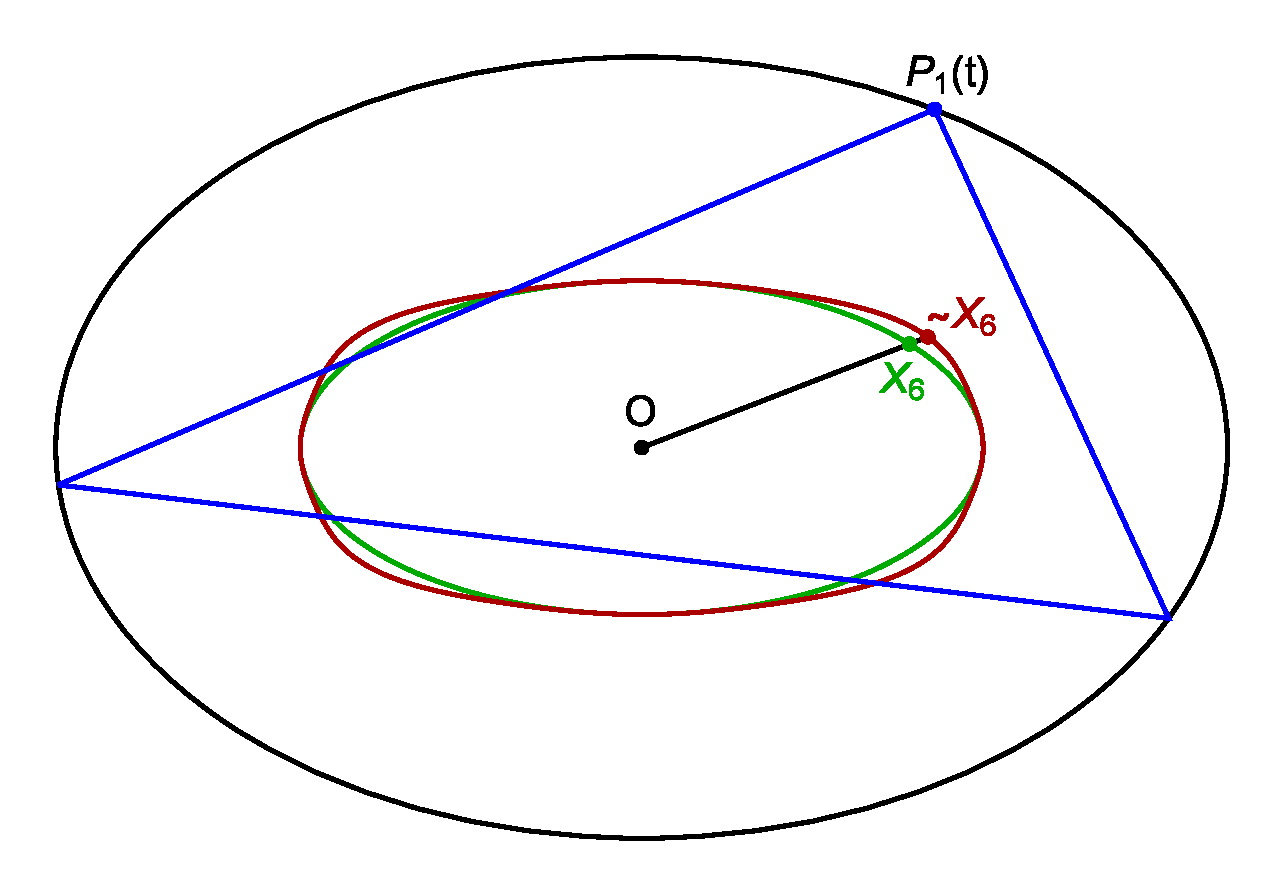
\includegraphics[width=.7\textwidth]{pics_05_090_symmedian}
    \caption{Over billiard 3-periodics (blue), the locus of the symmedian point $X_6$ is a quartic (green). At the billiard aspect ratio shown, it is visually identical to an ellipse. Also shown is a copy of the quartic (red) such that the distance to a best-fit ellipse (green) is scaled 1000 fold. \href{https://bit.ly/3hxOZoV}{Live}}
    \label{fig:05-locus-x6}
\end{figure}
%%% end X6

%%% BEGIN X11 and X100
\begin{figure}
    \centering
    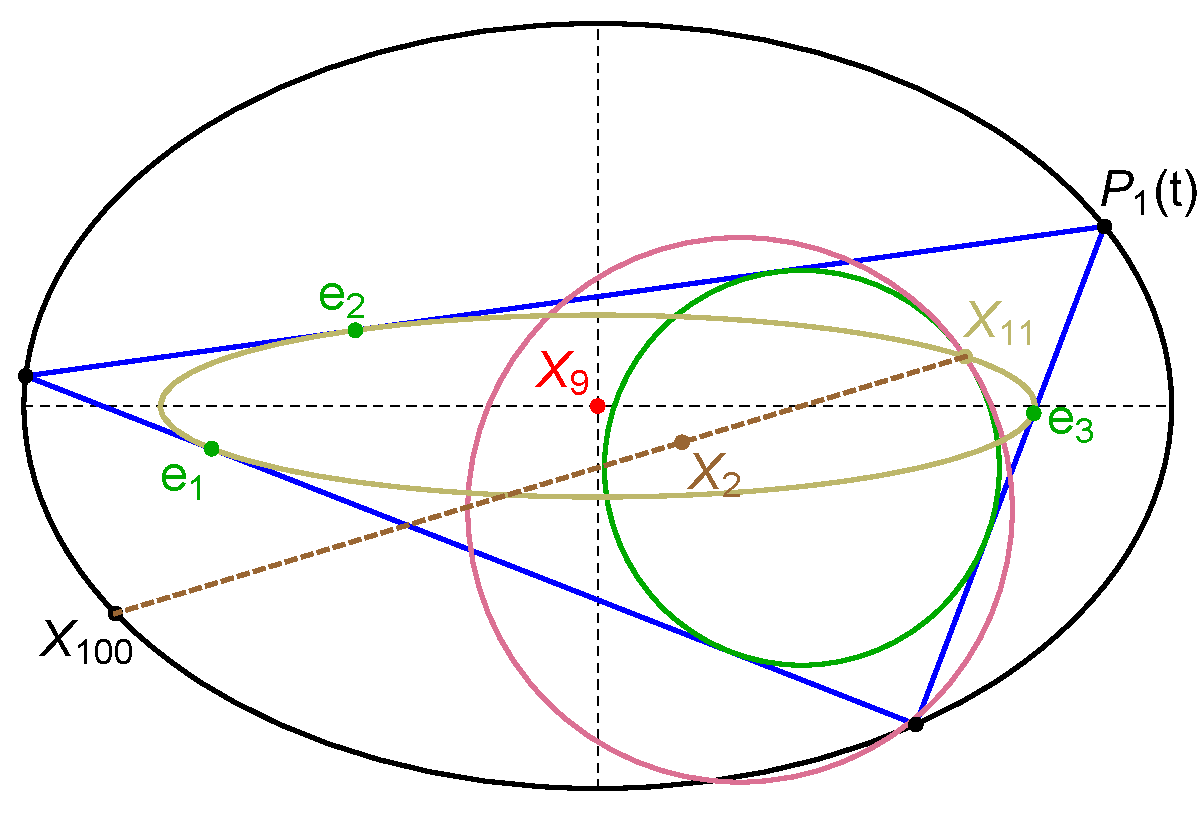
\includegraphics[width=.7\textwidth]{pics_05_080_feuerbach_loci.pdf}
    \caption{A billiard 3-periodic (blue). Also shown are the incircle (green) and 9-point circle (pink) which touch at the Feuerbach point $X_{11}$. Also shown is the latter's {\em anticomplement} $X_{100}$, and the three extouchpoints $e_1,e_2,e_3$. Over the billiard family, $X_{100}$ sweep the billiard while both $X_{11}$ and the extouchpoints sweep the caustic (though in opposite directions).
    % done
    \href{https://youtu.be/TXdg7tUl8lc}{Video},
    \label{fig:05-feuer-loci} \href{https://bit.ly/2S2LVqp}{Live}}
\end{figure}

\section{The locus of the Feuerbach point and its anticomplement}
\label{sec:05-x11-x100}

Referring to \cref{fig:05-locus-x11-x100}, the Feuerbach point $X_{11}$ is the single point of contact between incircle and 9-point circle \cite[X(11)]{mw}. $X_{11}$ is known to lie on the $X_{9}$-centered inconic, i.e., the  Mandart inellipse \cite[Mandart inellipse]{mw}. Since the latter is unique:

\begin{observation}
The confocal caustic is the stationary Mandart inellipse of billiard 3-periodics.
\end{observation}

Therefore:

\begin{proposition}
Over billiard 3-periodics, $X_{11}$ sweepts the confocal caustic.
\end{proposition}

The anticomplement of a point $P$ is its double-length reflection about the barycenter $X_2$, i.e., $A(P) = X_2+2 X_2-P$. Stille referring,  \cref{fig:05-locus-x11-x100}, $X_{100}$ is the anticomplement of $X_{11}$. This point is known to lie on (i) the circumcircle, (ii) the Steiner circumellipse (centered on $X_2$), and most relevantly here, (iii) on the $X_9$-centered circumellipse \cite[X(9)]{etc}. Since the latter is unique:

\begin{observation}
The elliptic billiard is the stationary $X_9$-centered circumconic of billiard 3-periodics.
\end{observation}

Therefore (proof is left as \cref{exe:05-x100}):

\begin{proposition}
Over billiard 3-periodics, the locus of $X_{100}$ is the elliptic billiard. It sweeps it in the direction opposite to that of the 3-periodic vertices along the billiard.
\label{prop:05-locus-x100}
\end{proposition}

The vertices of the so-called {\em extouch triangle} are the points of contact of the excircles with a triangle's sidelines \cite[Extouch triangle]{mw}. These are also known as {\em extouchpoints}. A known fact is that the Mandart inellipse (i.e., the caustic) touches a triangle's sidelines at the extouchpoints \cite[Mandart inellipse]{mw}. Therefore:

\begin{proposition}
Over billiard 3-periodics, the locus of the extouchpoints is the confocal caustic.
\end{proposition}

This is also illustrated in \cref{fig:05-locus-x11-x100}. A curious dynamic phenomenon is that while the extouchpoints follow the direction of motion of billiard 3-periodics along the outer ellipse (e.g., counter- or clockwise), $X_{11}$ rotates in the opposite direction; see this \href{https://bit.ly/2S2LVqp}{Live}.


%%% END X11 and X100

\section{A locus with singularities}

Loci considered thus far have been smooth, regular curves. Here we give an example of one with four corners. Recall that given a triangle $T$, the orthic triangle has vertices at the feet of $T$'s altitudes.

\begin{figure}
    \centering
    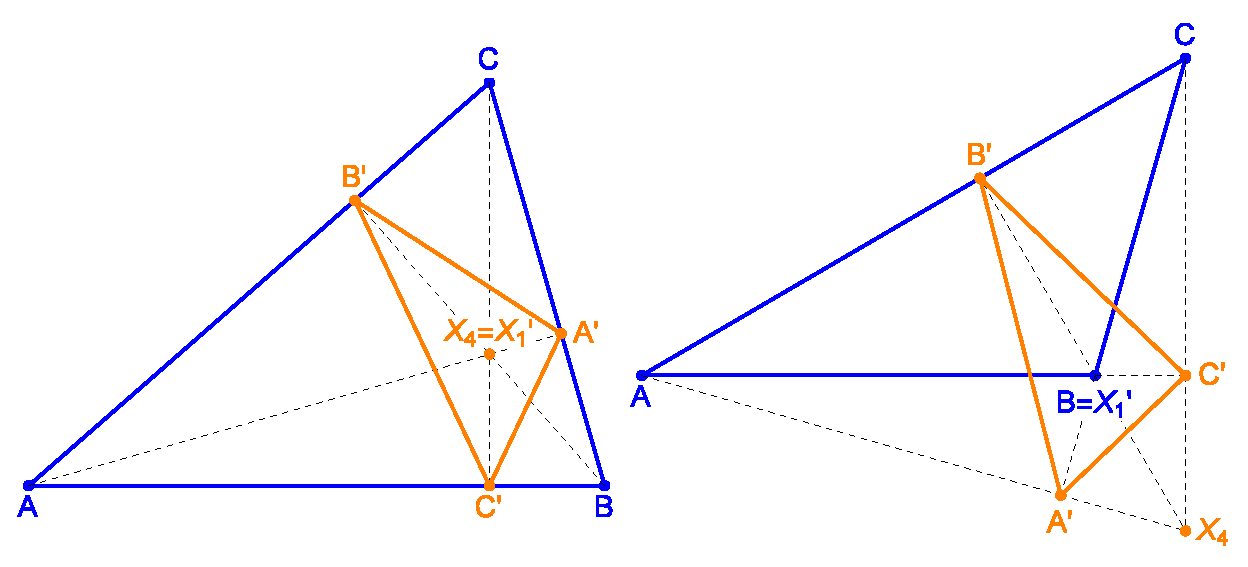
\includegraphics[width=.8\textwidth]{pics_05_140_orthic_incenter}
    \caption{\textbf{Left}: the orthic triangle (orange) is shown of an acute reference triangle $T$ (blue), for with an interior orthocenter $X_4$. In this case, the orthic incenter $X_1'$ coincides with $X_4$. \textbf{Right}: When $T$ (blue) is obtuse, $X_4$ is exterior. Furthermore, two orthic vertices are outside of $T$ and $X_1'$ coincides with the obtuse vertex, $B$ in the picture. \href{https://youtu.be/-bLuvICzmqM}{Video}}
    \label{fig:05-orthic-incenter}
\end{figure}

Referring to \cref{fig:05-orthic-incenter}, 
it is easy to see that if a triangle $T$ is acute (resp. obtuse), all three vertices (only one vertex) of the orthic will lie on a sideline. In the obtuse case, the other two will lie on extensions of two sidelines, i.e., they will be exterior to $T$.

An interesting result, mentioned in \cite[Chapter 1]{coxeter67}, is the ``switching'' behavior of the incenter of the orthic triangle:

\begin{lemma}
If a triangle is acute (resp. obtuse), the incenter of the orthic will coincide with the orthocenter (resp. the obtuse vertex of $T$).
\label{lem:05-pinned}
\end{lemma}

Recall that for billiard 3-periodics to include obtuse triangles, $a/b>\alpha_4$; see \cref{prop:05-alpha4}. Referring to
\cref{fig:05-orthocenter-loci}:

% \includegraphics[trim={left bot right upper},clip]
\begin{figure}
    \centering
    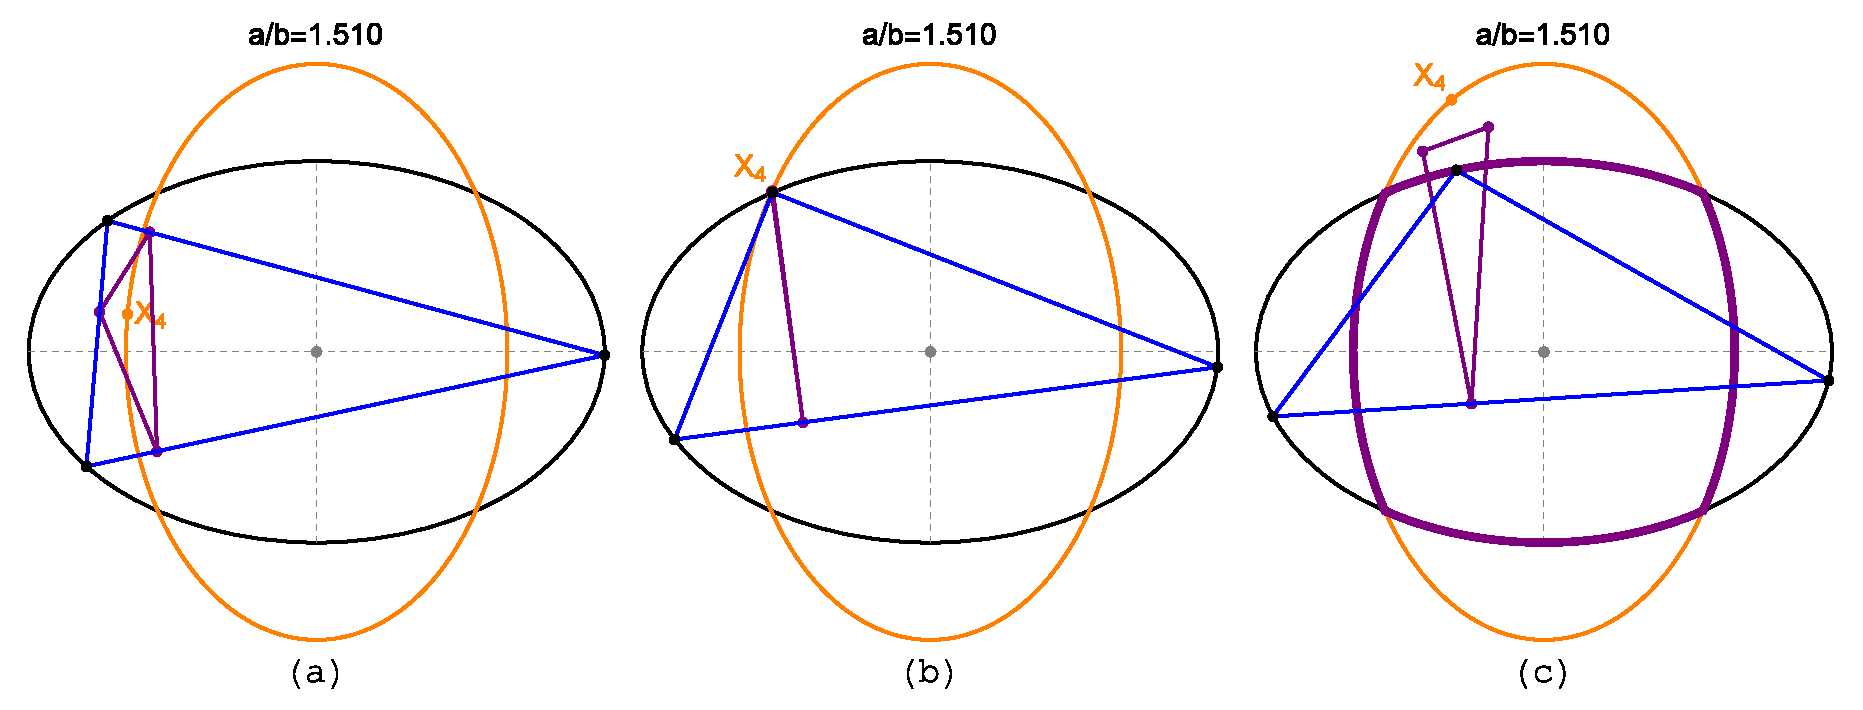
\includegraphics[trim={0 0 0 20},clip,width=\textwidth]{pics_05_120_ort_loci_kink.eps}
    \caption{From left to right: the orthic triangle (purple) of billiard 3-periodics (blue) is shown at 3 different positions. The locus of $X_4$ (orange ellipse) intersects the billiard, i.e., $a/b>\alpha_4$. When a 3-periodic is acute (left), the orthic incenter coincides with $X_4$. When it is a right triangle (middle), $X_4$ is on the elliptic billiard and the orthic is a degenerate segment. When it is obtuse (right), the orthic incenter remains ``pinned'' to the obtuse vertex. The end result is that the locus of the orthic incenter is a quadrilateral with four elliptic arcs (thick purple, right) with four corners.  \href{https://youtu.be/3qJnwpFkUFQ}{Video}, \href{https://bit.ly/33TVjit}{Live}}
    \label{fig:05-orthic_incenter_locus}
\end{figure}

\begin{corollary}
If $a/b>\alpha_4$, the locus of the incenter of the orthic triangle of billiard 3-periodics is an elliptic arc ``quadrilateral'' with four corners.
\end{corollary}

%%% begin self-inter

\section{A self-intersecting locus}

Consider the curious case of a triangle center which is the isogonal conjugate of the Feuerbach point, listed on \cite{etc} as $X_{59}$. We revisit its intriguing locus, shown previously in \cref{fig:01-intouch-x59}(right).

This is a continuous curve with four self-intersections, internally tangent to the elliptic billiard on its four vertices independently of $a/b$; see \cref{fig:05-x59-locus}. Since it intersects a line parallel to and infinitesimally away from either axis at six points, its degree must be at least 6.

We propose leave it as a research question (below) the derivation of this locus (as an implicit and/or parametric equation) and of its critical points. 

\begin{figure}
    \centering
    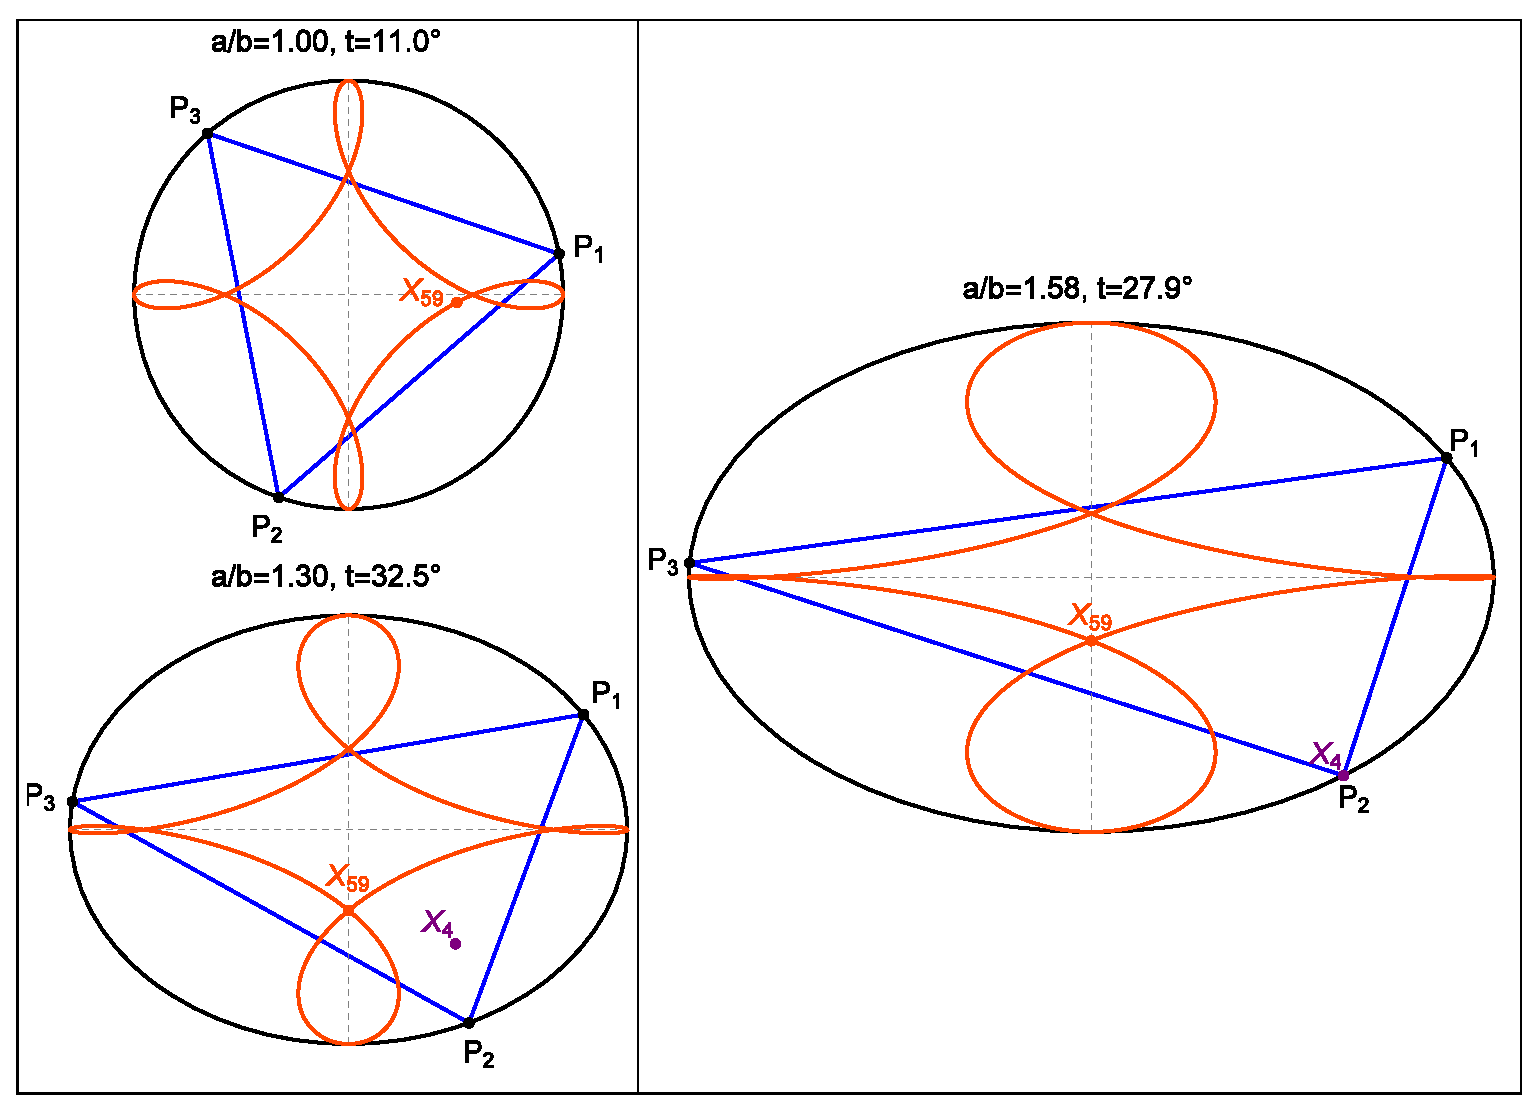
\includegraphics[width=\textwidth]{pics_05_160_x59_center}
    \caption{Over billiard 3-periodics, the locus of $X_{59}$ is a continuous curve with four self-intersections, tangent to the billiard at its four vertices. \textbf{Top Left}: if $a/b$ is slightly above 1, the locus of  $X_{59}$ is nearly four-fold symmetric. Not shown: if $a/b=1$, $X_{59}$ will be on the line at infinity. \textbf{Bottom Left}: An acute 3 periodic $a/b<\alpha_4$, and an acute 3-periodic. \textbf{Right}: a right-angle 3-periodic in an $a/b>\alpha_4$ elliptic billiard. \href{https://youtu.be/pl_PqSuhlx0}{Video}, \href{https://bit.ly/3fvDlZd}{Live}}
    \label{fig:05-x59-locus}
\end{figure}

%%% end self-inter

%%% begin non-compact
\section{A non-compact locus}

Given a triangle $T$, the {\em tangential triangle} $T'$ has sides tangent to the circumcircle at the vertices \cite[Tangential triangle]{mw}. Notice $T'$ is unbounded for a right triangle since the hypotenuse is a diameter of the circumcircle. Consider a smooth deformation of an acute triangle to an obtuse one: one of the vertices of the tangential triangle will undergo a discontinuous jump.

Recall that the family of billiard 3-periodics with $a/b>\alpha_4$ (resp. $a/b<\alpha_4$) contains both acute and obtuse (resp. only acute) triangles. Therefore the family of $T'$ will (will not) undergo discontinous jumps, and the locus of triangle centers thereof will be non-compact (resp. compact).

As an example, consider the locus of the circumcenter of the tangential triangle, listed as $X_{26}$ in \cite{etc}. It can be shown it is non-elliptic. As shown in \cref{fig:05-locus-x26}, it is non-compact (resp. compact) when $a/b>\alpha_4$ (resp. $a/b<\alpha_4$). In the former case, the locus is compactified by an inversion with respect to the center.

\begin{figure}
    \centering
    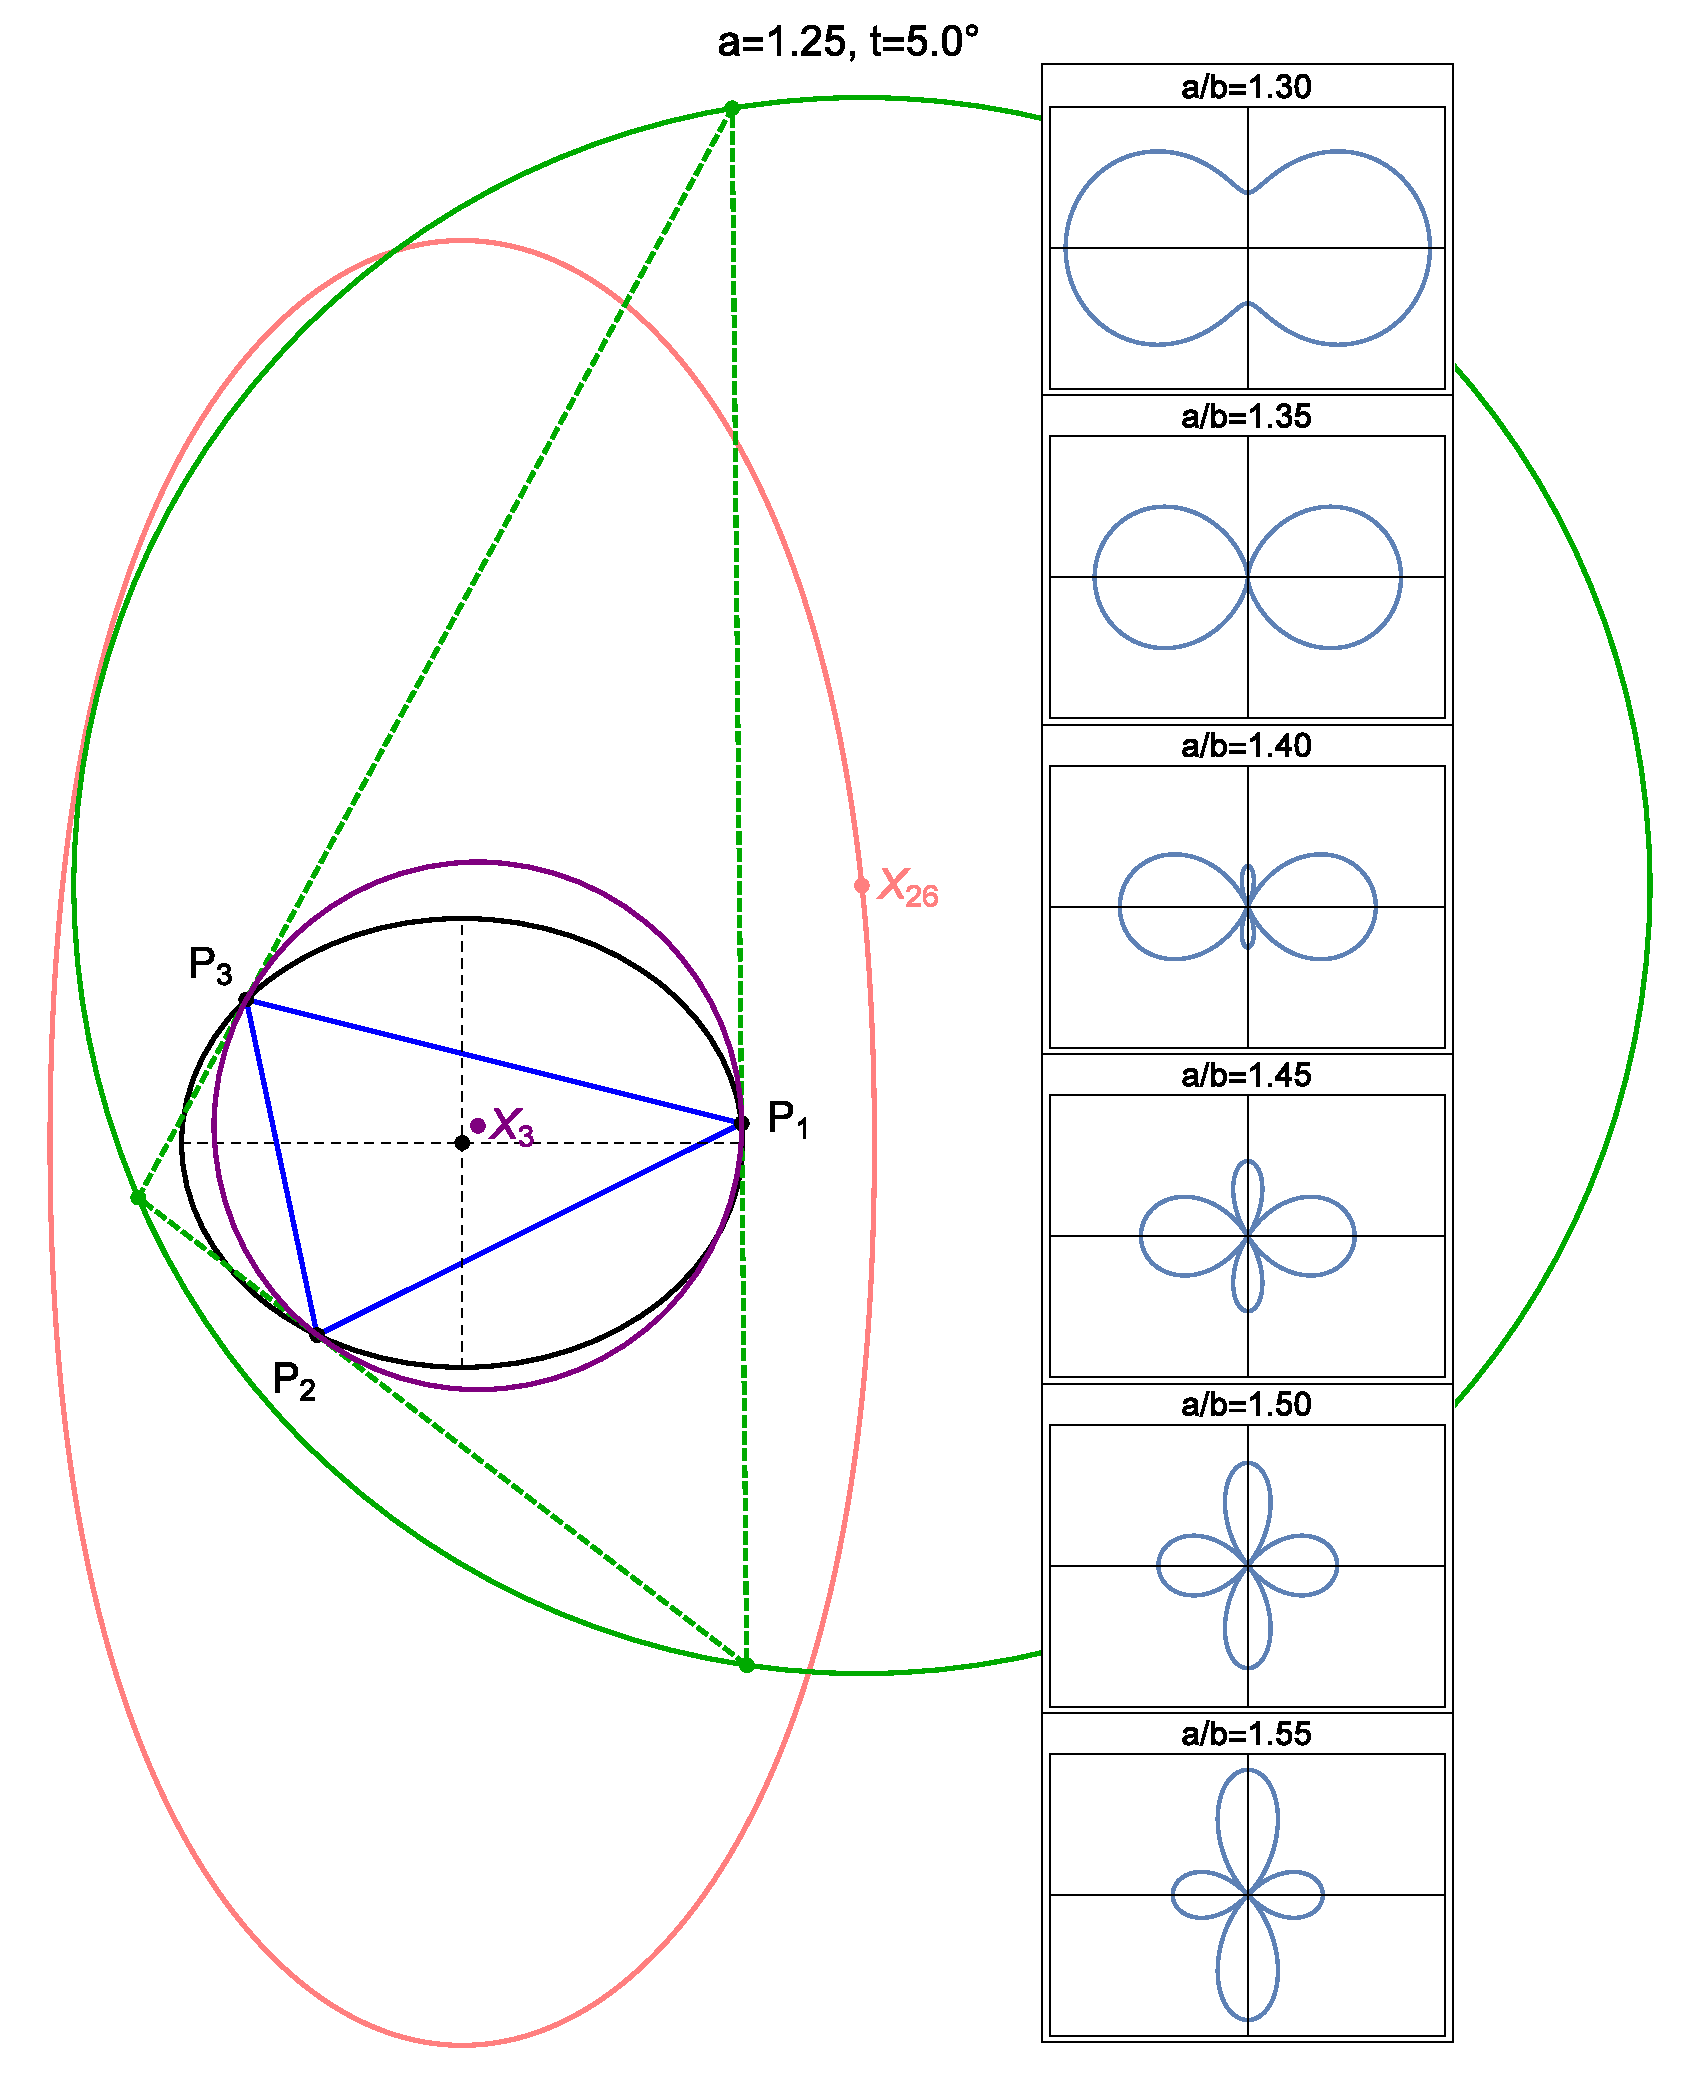
\includegraphics[width=\textwidth]{pics_05_170_x26}
    \caption{\textbf{Left:} The tangential triangle (dashed green) is bounded by the tangents to the circumcircle (purple)  at the vertices of a reference triangle (blue), in this case a 3-periodic in an $a/b<\alpha_4$ elliptic billiard. The center of the tangential circumcircle (green) is known as $X_{26}$. In the case shown, all 3-periodics are acute, therefore the locus of $X_{26}$ is compact (and non-elliptic). \textbf{Right inset:} the image of the (non-compact) locus of $X_{26}$ under an inversion with respect to a circle concentric with the billiard, for various values of $a/b{\geq}\alpha_4$. Origin crossings are equivalent to $X_{26}$ at infinity. \href{https://bit.ly/3446TYF}{Live 1 (compact)}, \href{https://bit.ly/3hMiTpT}{Live 2 (non-compact)}}
    \label{fig:05-locus-x26}
\end{figure}

%%% end non-compact

%%% begin golden
\section{A golden locus}
\label{sec:05-golden-locus}

The circumcenter of the excentral Triangle is known as the {\em Bevan point} $X_{40}$ \cite{etc}. The following was shown in \cite{garcia2020-ellipses}:

\begin{proposition}
Over billiard 3-periodics, the locus of $X_{40}$ is an ellipse similar to a rotated copy of the elliptic billiard. Its semi-axes are given by 
%
\begin{equation*}
    a_{40}=c^2/a,\;\;\; b_{40}=c^2/b.
\end{equation*}
\end{proposition}

\begin{corollary}
At $a/b=\sqrt{2}$, the top and bottom vertices of the locus of $X_{40}$ touches the top and bottom vertices of the elliptic billiard.
\label{cor:05-x40-tangent}.
\end{corollary}

Referring to \cref{fig:05-x40-golden}, the following is a harmonious fact associated with the locus of $X_{40}$:

\begin{corollary}
At $a/b = (1+\sqrt{5})/2=\varphi$, the Golden Ratio, the locus of $X_{40}$ is identical to a $90^\circ$-rotated copy of the elliptic billiard.
\label{cor:05-x40-golden}
\end{corollary}

\begin{figure}
    \centering
    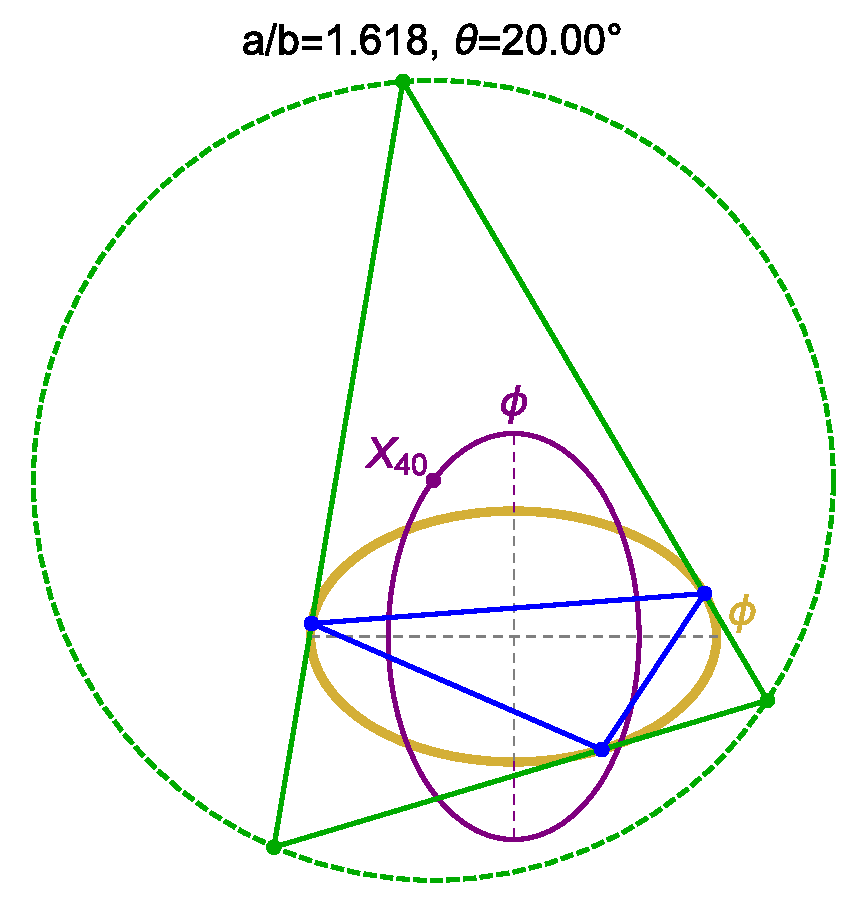
\includegraphics[width=.7\textwidth]{pics_05_180_x40}
    \caption{A 3-periodic (blue) is shown within an $a/b=\varphi$ elliptic billiard (gold) as well as its excentral triangle (green). At this aspect ratio, the locus of the Bevan point $X_{40}$ (purple) is a $90^\circ$-rotated copy of the billiard. Recall this point is the circumcenter of the excentral triangle. \href{https://youtu.be/rg28gGr-Qeo}{Video}, \href{https://bit.ly/3f4eQ6e}{Live}}
    \label{fig:05-x40-golden}
\end{figure}

%%% end golden

\section{When the billiard is swept non-monotonically}
\label{sec:05-non-monotonic}

In \cref{prop:05-locus-x100}, we saw that $X_{100}$ sweeps the elliptic billiard in the direction opposite to the motion of billiard 3-periodic vertices.

The next triangle center on \cite{etc} which is on the $X_9$-centered circumconic is $X_{88}$, known to be collinear with $X_1$ and $X_{100}$. Assume a monotonic traversal of billiard 3-periodic vertices along the billiard. It turns out at a certain aspect ratio, the ``motion'' of $X_{88}$ can be made to stop. 

\begin{proposition}
At $a/b=\alpha_{88}$, the y velocity of $X_{88}$ vanishes when the 3-periodic is a sideways isosceles, where 
\[\alpha_{88}=(\sqrt{6+2\sqrt{2}}\,)/2\simeq{1.485} \]
\end{proposition}

\begin{proof}
Parametrize a 3-periodic vertex $P_1(t)=[a \cos{t},b \sin{t}]$. At $t=0$, $P_1=(a,0)$ it can be easily checked that $X_{88}=(-a,0)$. Solve $y_{88}'(t)|_{t=0}=0$ for $a/b$. After some algebraic manipulation, this equivalent to solving $4x^4-12x^2+7=0$, whose positive roots are $(\sqrt{6\pm 2\sqrt{2}}\,)/2$. $\alpha_{88} $ is the largest of the two.
\end{proof}

Indeed, there are three types of $X_{88}$ motion with respect to $P_1(t)$: (i) $a/b<\alpha_{88}$: monotonic and opposite to $P_1(t)$; (ii) $a/b=\alpha_{88}$: monotonic and opposite, but with full stop at the billiard major vertices; (iii) $a/b<\alpha_{88}$: non-monotonic, containing two retrograde phases.

An equivalent statement, illustrated in \cref{fig:05-x88-envelope}, is that the line family $X_1 X_{100}$ is instantaneously tangent to its {\em envelope} at $X_{88}$. Referring to Figure~\ref{fig:05-x88-envelope}:

\begin{proposition}
Over billiard 3-periodics, the envelope of $X_1 X_{100}$ is (i) entirely inside, (ii) touches at vertices of, or (iii) intersects the billiard, for $a/b$ (i) less than, (ii) equal to, or (iii) greater than $\alpha_{88}$, respectively. 
\label{prop:05-x88-env}
\end{proposition}

Interestingly:

\begin{proposition}
The motion of $X_{88}$ is instantaneously (i) opposite to $P_1$, (ii) stationary, or (iii) in the direction of $P_1$, if the tangency $E$ of $X_1 X_{100}$ with the envelope lies inside, on, or outside the billiard.
\label{prop:05-x88-envelope}
\end{proposition}

\begin{figure}
    \centering
    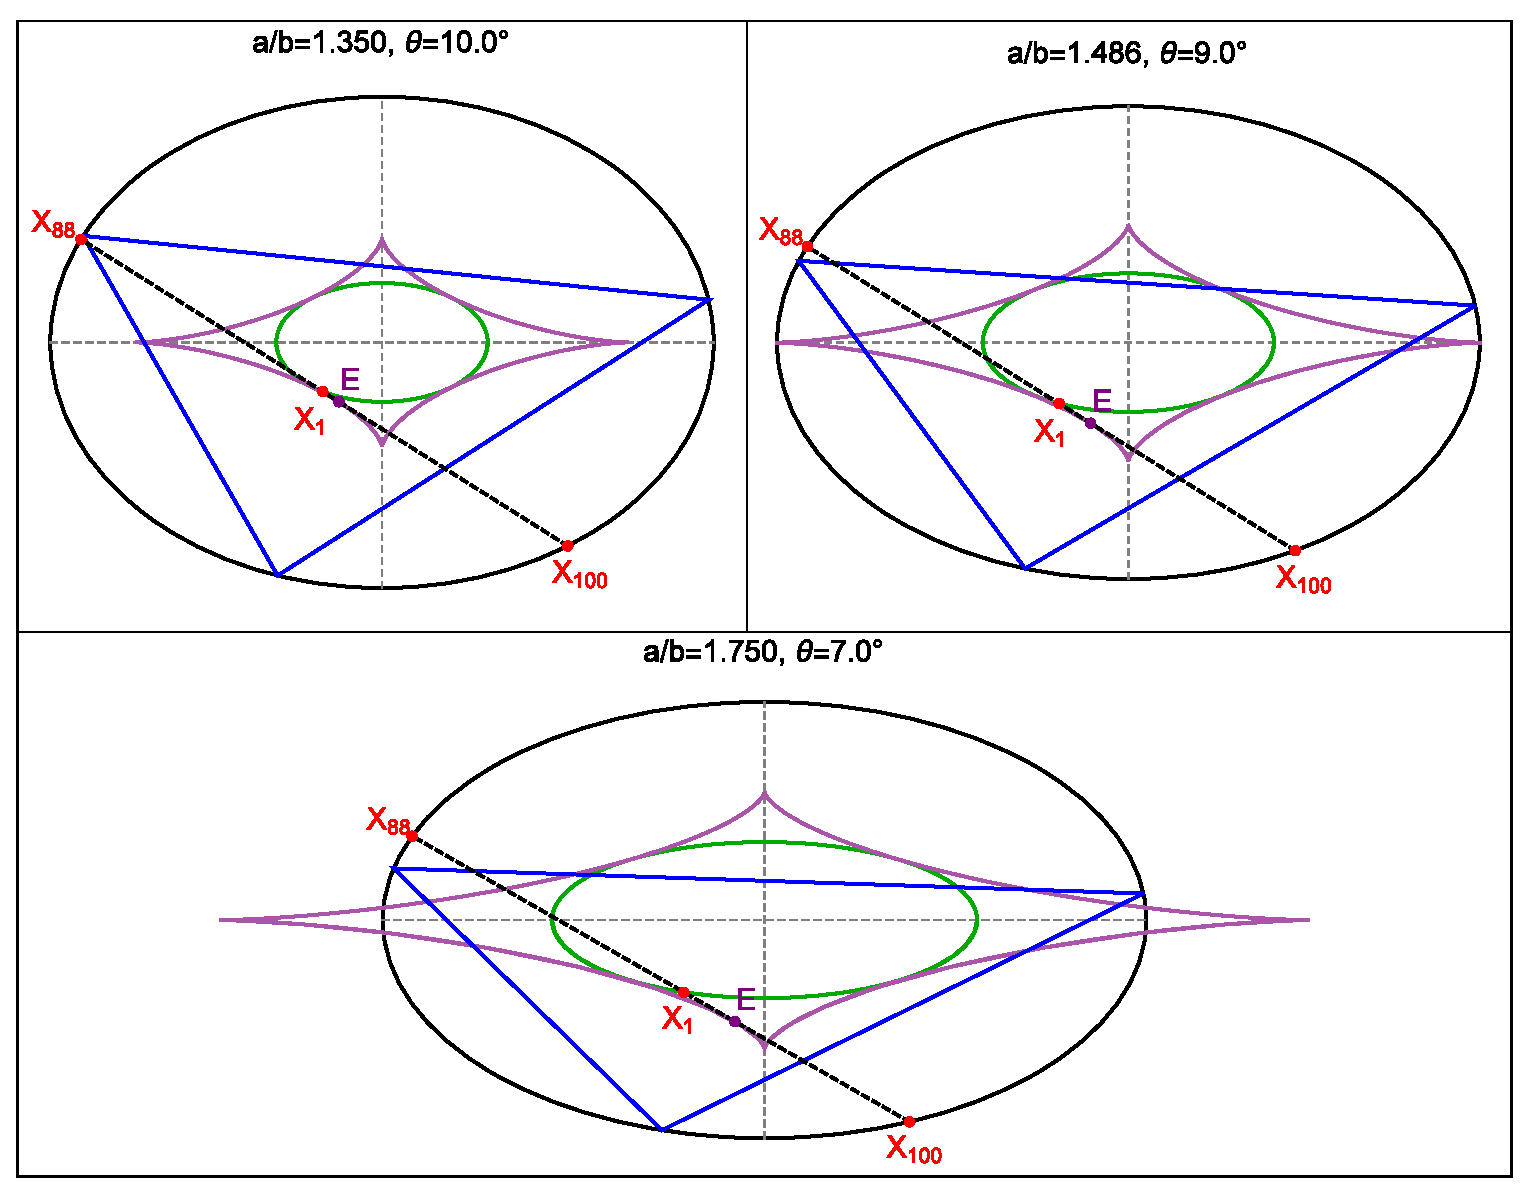
\includegraphics[width=\textwidth]{pics_05_190_trio}
     \caption{Collinear points $X_1,X_{100},X_{88}$ shown in an elliptic billiard with $a/b$ (i) less than (top-left), (ii) equal to (top-right), or (iii) greater than (bottom), $\alpha_{88}{\simeq}1.486$. The motion of $X_{88}$ relative to 3-periodic vertices will be: (i) monotonic and opposite to the vertices, (ii) monotonic and opposite but will full stops at the vertices, and (iii) non-monotonic. The envelope (purple) of line  $X_1 X_{100}$ intersects the billiard if $a/b>\alpha_{88}$ (bottom). The motion of $X_{88}$ is instantaneously (i) opposite to $P_1$, (ii) stationary, or (iii) in the direction of $P_1$, if the tangency $E$ of $X_1 X_{100}$ with the envelope lies inside, on, or outside the billiard. \href{https://youtu.be/nJLp--JjDZU}{Video}, \href{https://bit.ly/3hKicgM}{Live}}
    \label{fig:05-x88-envelope}
\end{figure}

\section{The dance of the swans}
\label{sec:05-swans}

Some 50+ triangle centers are listed under \cite[X(9)]{etc} which by definition lie on the $X_9$-centered circumconic, show in this \href{https://youtu.be/JdcJt5PExsw}{Video}. We call such centers $X_9$ ``swans'' since over billiard 3-periodics they swim along the margins of an elliptic ``pond''. The first four on \cite{etc} are $X_k$, $k=$88, 100, 162, and 190.

Above we saw that the motion of $X_{100}$ is ``monotonic'' whereas that with $a/b>\alpha_{88}$ that of $X_{88}$ isn't. The next two swans in \cite{etc} are $X_{162}$ and $X_{190}$. 

\begin{proposition}
\label{prop:05-x162}
The motion of $X_{162}$ with respect to $P_1(t)$ is non-monotonic if $a/b>\alpha_{162}$ where $\alpha_{162}{\simeq}1.1639$ is the only positive root of:
\[ 5 x^8 + 3 x^6 - 32 x^4 + 52 x^2 - 36 \]
\end{proposition}

\begin{proof}
The trilinear coordinates of $X_{162}$ are given by
{\small 
\[  \frac {1}{ \left( s_2^{2}-  s_3^{2} \right)  \left( s_2^{2}+ s_3^{2}-
s_1^{2} \right) } :  \frac {1}{ \left( s_3^{2}-  s_1^{2} \right)  \left( s_3^{2}+ s_1^{2} -
s_2^{2} \right) }:\frac {1}{ \left( s_1^{2}-  s_2^{2} \right)  \left( s_1^{2}+ s_3^{2} -
s_3^{2}\right) }\cdot
\]
}

We use the standard parametrization for vertices of the confocal family found in \cref{sec:02-confocal-standard-param}. Using the trilinear coordinates above, we have   $X_{162}(t)=(x_{126}(t), y_{126}(t))$ 
  At $t=\frac{\pi}{2}$, $P_1=(0,b)$ and   $X_{162}(\frac{\pi}{2})= (0,b)$.
  
  Solve $x_{162}'(t)|_{t=\frac{\pi}{2}}=0$ for $a/b$. After some long algebraic symbolic manipulation, this is equivalent to solving $5 x^8 + 3 x^6 - 32 x^4 + 52 x^2 - 36=0$, whose positive roots is $  \alpha_{162} \simeq 1.16369.$
\end{proof}

Since $\alpha_{88}>\alpha_{162}$, setting $a/b>\alpha_{88}$ implies both centers will move non-monotonically. Curiously:

\begin{proposition}
With $a/b>1$, $X_{88}$ and $X_{162}$ never coincide. Therefore over the billiard 3-periodic family, they never cross each other.
\end{proposition}

\begin{proof}
Consider an elementary triangle $P_1=(-1,0)$, $P_2=(1,0)$ and $P_3=(u,v)$. Obtain cartesian coordinates for $X_{88}$ and $X_{162}$ using their trilinears. The equation $X_{88}=X_{162}$ is given by two algebraic equations $F(u,v,s_1,s_2)=G(u,v,s_1,s_2)=0$ of degree 17 with   $s_1=\sqrt{(u-1)^2+v^2}=\mid P_3-P_2\mid$ and $s_2=\sqrt{(u+1)^2+v^2}=\mid P_2-P_1\mid$.
Particular solutions of these equations are    equilateral triangles with $P_3=(0,\pm \sqrt{3})$ in which case $X_{88}$ and $X_{162}$ go to infinity, i.e., these centers can never meet with $a/b>1$.
%\textcolor{red}{sketch. A figura esta com %cores erradas. Vou corrigir mas nao consigo %agora pois o meu inkscape nao funciona mais %com a atualizacao do mac.}
\end{proof}

\begin{figure}
    \centering
    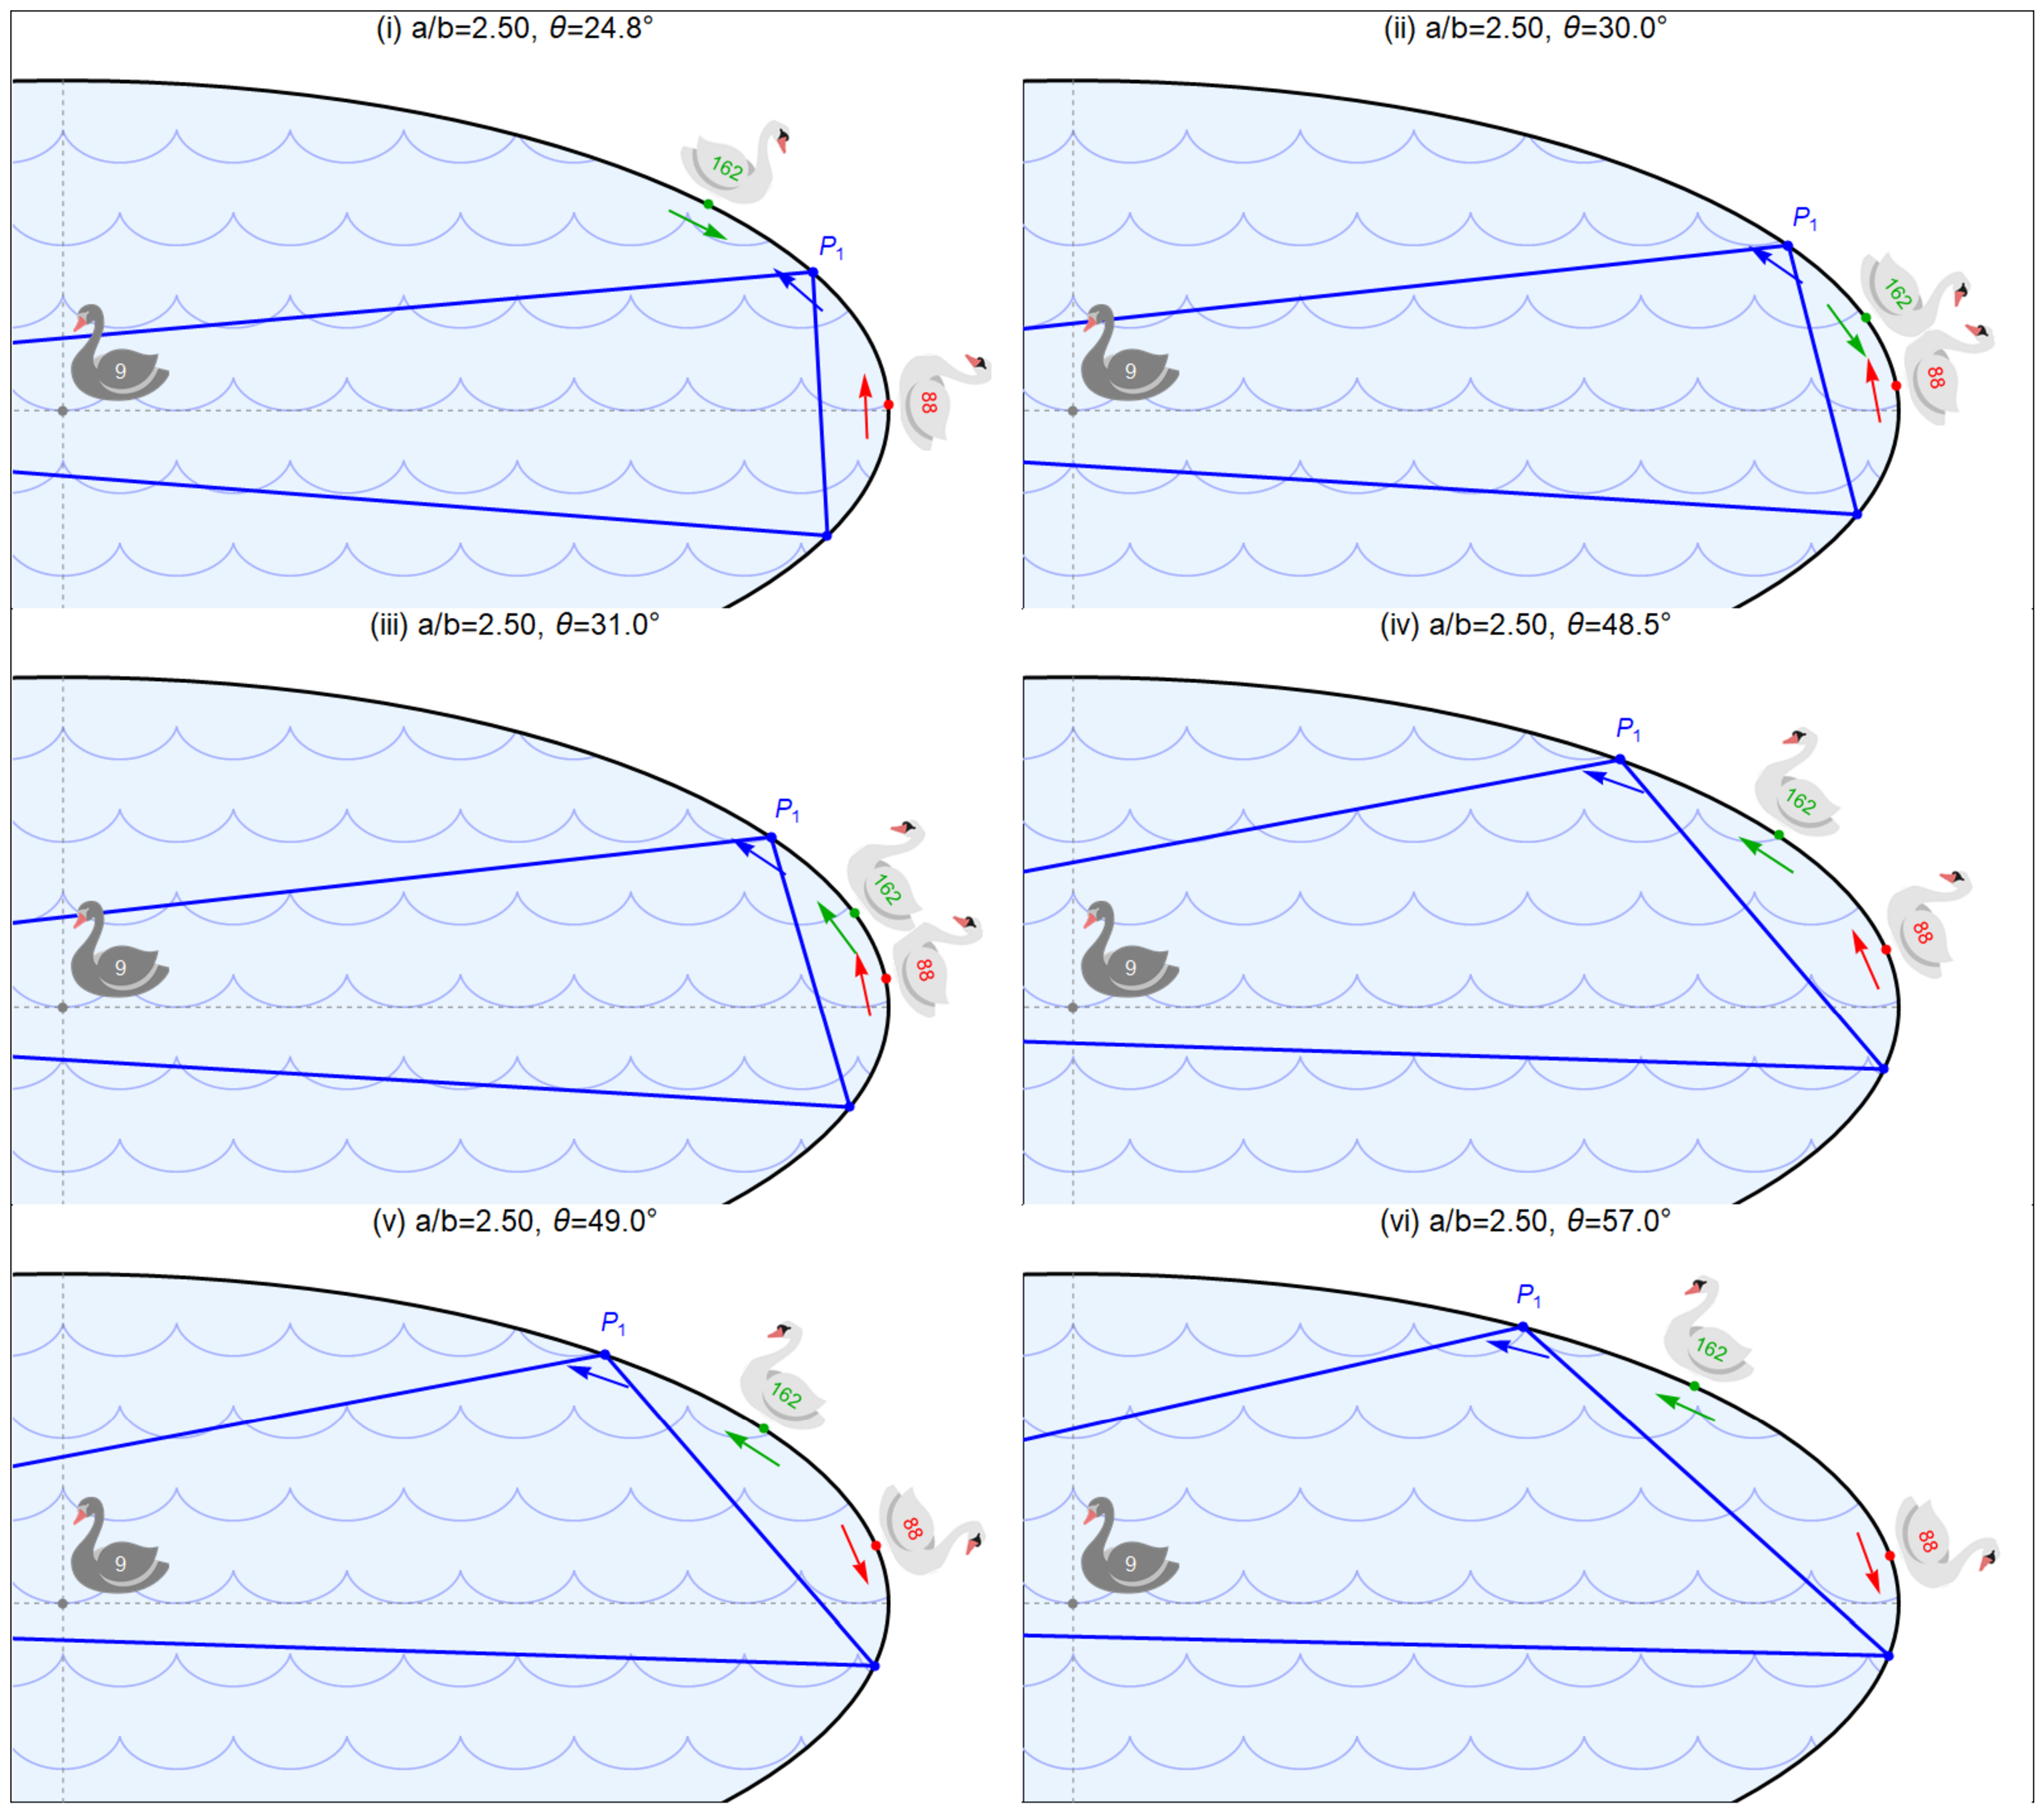
\includegraphics[width=\linewidth]{pics_05_200_swan_frames}
    \caption{The dance of swans $X_{88}$ and $X_{162}$ along the margins of an elliptic pond. (i) while $P_1$ moves CCW, $X_{88}$ and $X_{162}$ approach each other; (ii) at their closest, they almost kiss. (iii) Suddenly, $X_{162}$ reverses course, (iv) and a short-lived same-direction pursuit ensues. (v) An unswooned $X_{88}$ also changes course, (vi) with now both swimming away from each other. The duo meets again on 2nd, 3rd and 4th quadrants, where the dance steps are played back in alternating forward and backward order. A black mittenswan guards his clutch at the center of the lake. \href{https://youtu.be/ljGTtA1x-Sk}{Video}, two \href{https://bit.ly/3f6M9Wh}{Live} swans, four \href{https://bit.ly/3oDhMdd}{Live} swans.}
    \label{fig:x88-x162}
\end{figure}

The joint motion of $P_1(t)$, $X_{88}$, and $X_{162}$ can be visualized on the surface of a torus where the meridians (circles around the smaller radius) correspond to a given $t$ and the parallels represent a fixed location on the billiard boundary. As shown in \cref{fig:05-3d-torus}, the curves for $X_{88}$ and $X_{162}$ are thrice-winding, though never intersecting.

\begin{figure}
    \centering
    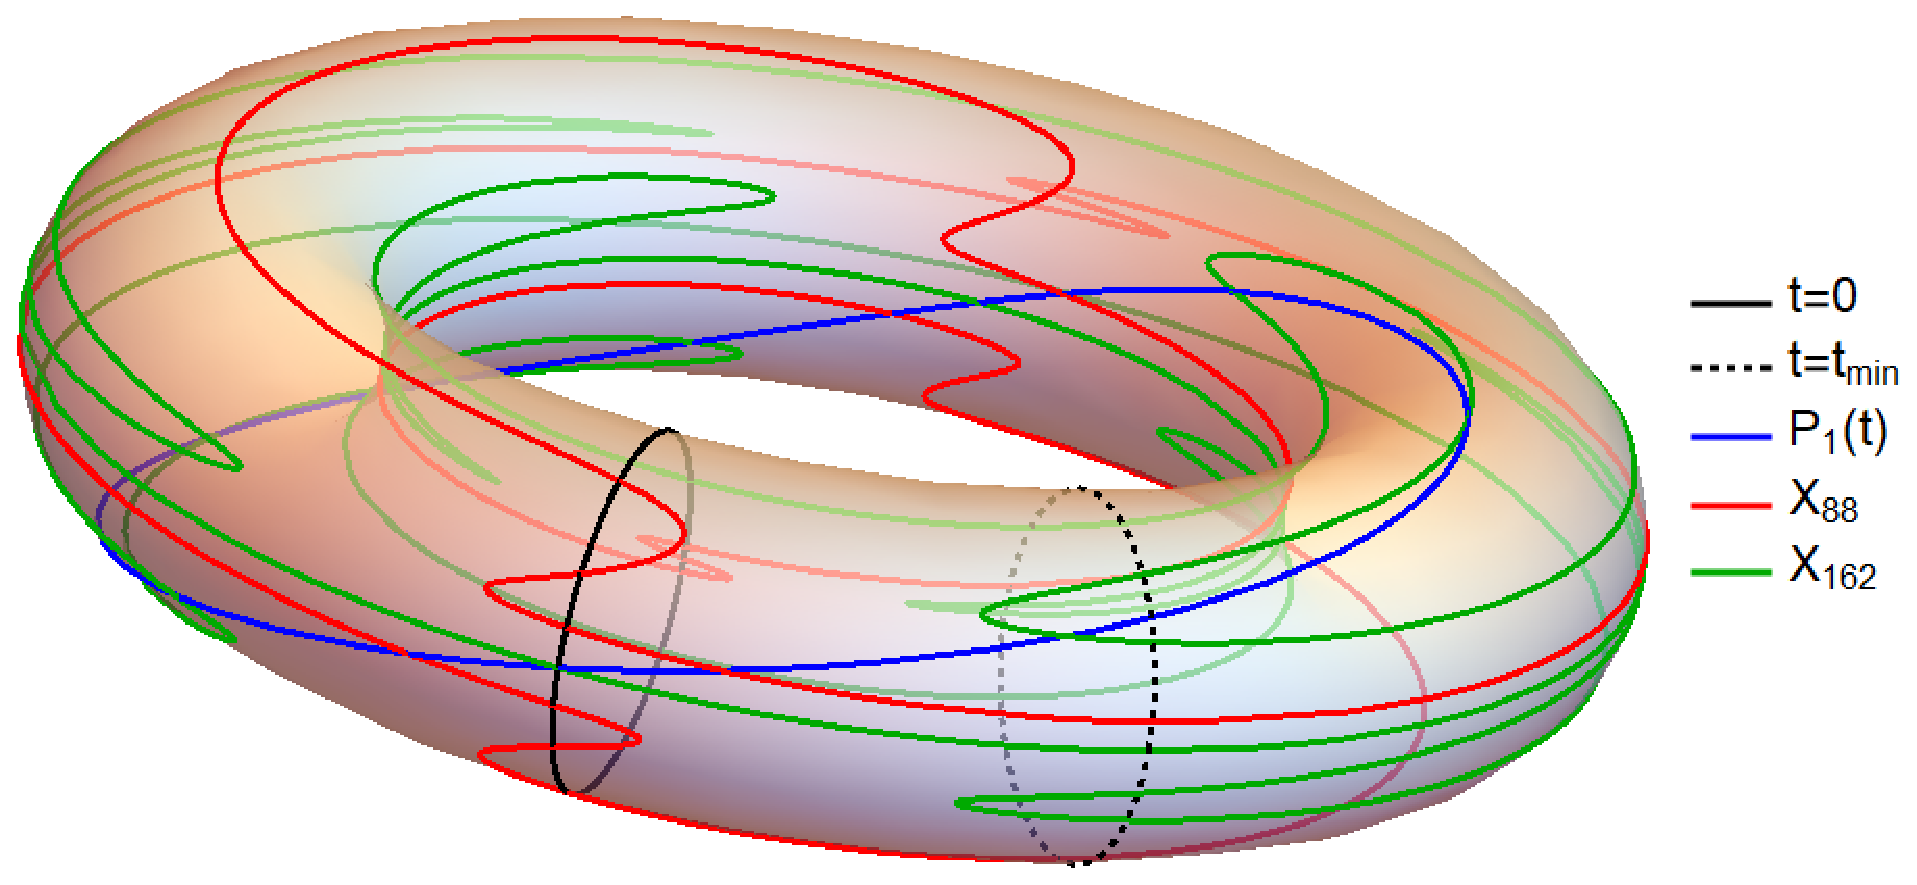
\includegraphics[width=\textwidth]{pics_05_210_torus_x88_x126_cropped}
    \caption{The coordinated motion of $P_1(t)$ (blue), $X_{88}$ (red) and $X_{162}$ (green) on the surface of a translucent torus, whose (i) meridians represent position along the elliptic billiard, and (ii) parallels the family parameter $t$. Notice the green and red curves are non-monotonic around the torus but never cross each other. A solid black meridian is wound at $t=0$ and a dashed one appears at one of the 12 instants of closest distance between $X_{88}$ and $X_{162}$, see \cref{que:05-x88-x162}.}
    \label{fig:05-3d-torus}
\end{figure}

\section{Locus of vertices of derived triangles}

A few triangles derived from billiard 3-periodics are shown in \cref{fig:05-derived-isosceles}. For their definitions see \cref{app:app-triangle} and \cite{mw}.

\begin{figure}
    \centering
    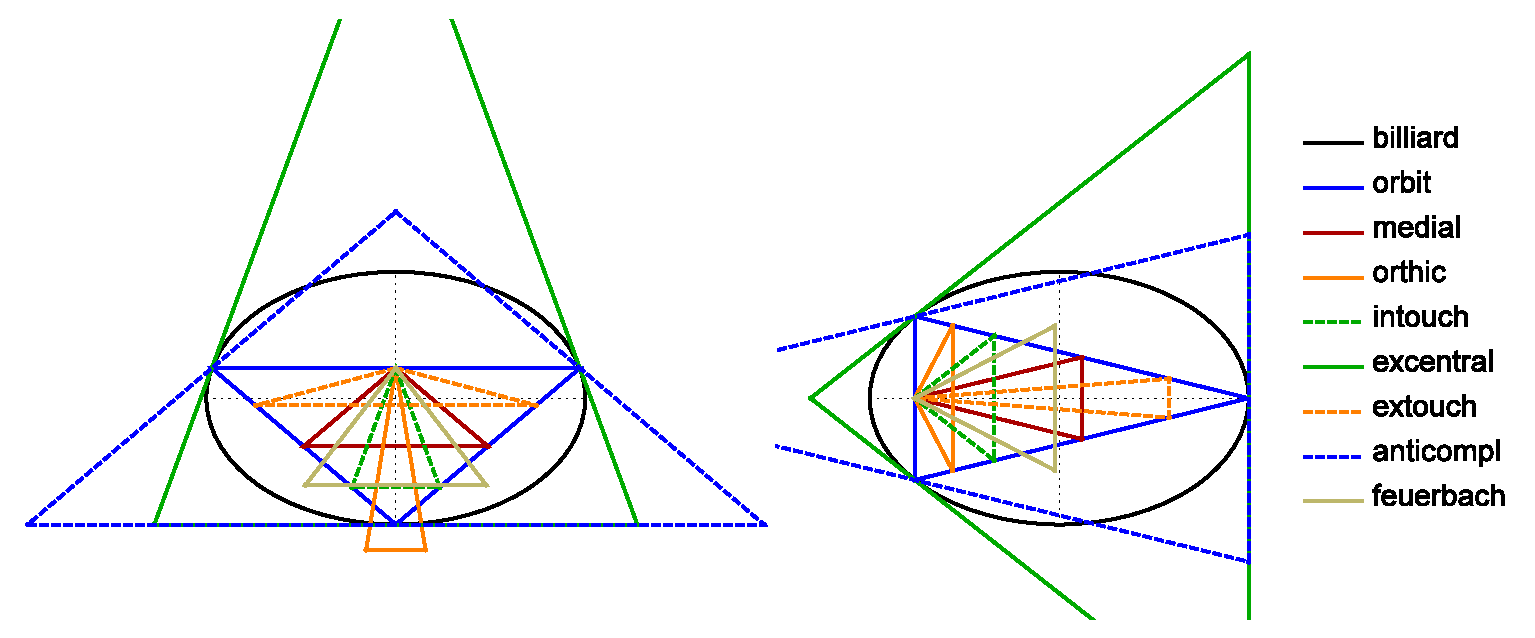
\includegraphics[width=\textwidth]{pics_05_100_confocal_derived}
    \caption{Triangles derived from an isosceles billiard 3-periodic (blue). These contain one vertex on the axis of symmetry. \href{https://youtu.be/xyroRTEVNDc}{Video}, \href{https://bit.ly/3fyylD0}{Live}}
    \label{fig:05-derived-isosceles}
\end{figure}

Mentioned in \cref{chap:01-intro} was an early experiment which showed that over billiard 3-periodics, the locus of the vertices of the intouch triangle (i.e., the intouchpoints) is a 2-lobed, self-intersect curve; see \cref{fig:01-intouch-x59}.

As shown in \cref{fig:05-locus-x11-x100}, the loci of vertices of some other triangles derived from billiard 3-periodics aren't ellipses. A noteworthy exception is the extouch triangle, mentioned above.

\begin{figure}
    \centering
    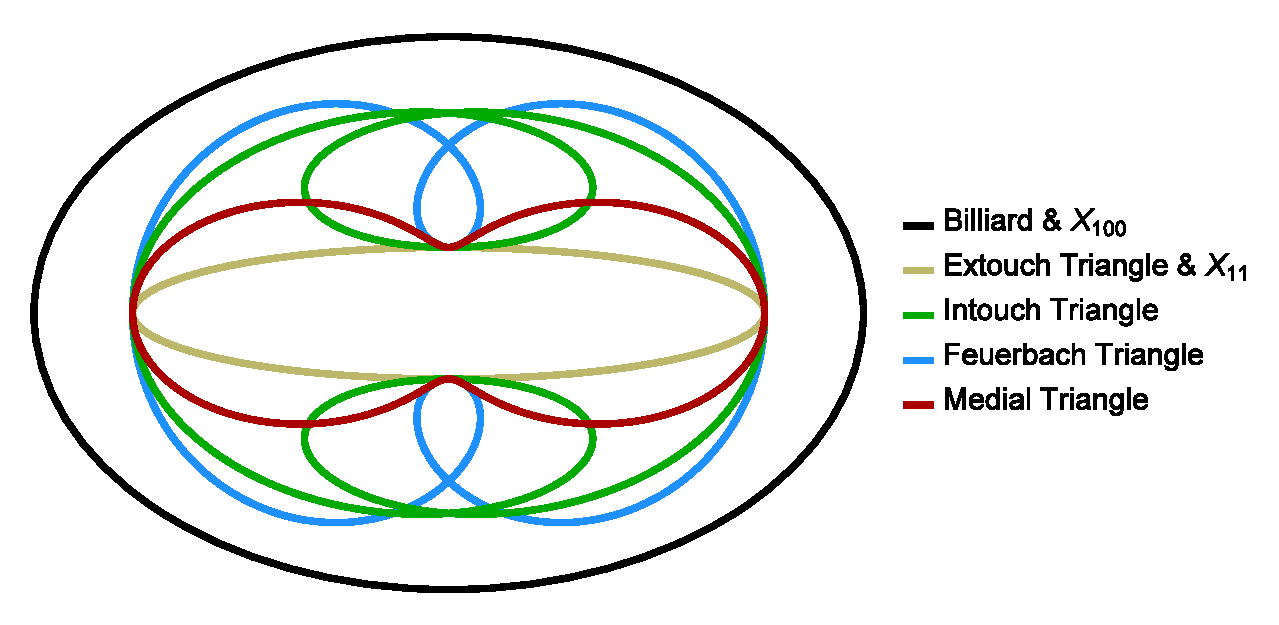
\includegraphics[width=\textwidth]{pics_05_070_non_elliptic}
    \caption{Non-elliptic loci of the vertices of triangles derived from billiard 3-periodics: the (i) intouch (green), (ii) Feuerbach (not to be confused with the Feuerbach {\em point}) (blue), (iii) medial (red), triangles. A noteworthy excpetion is the extouch triangle (light brown), whose vertices sweep the confocal caustic.
     \href{https://youtu.be/OGvCQbYqJyI}{Video}, \href{https://bit.ly/3orrSxQ}{Live}}
    \label{fig:05-locus-x11-x100}
\end{figure}

As said above, $X_{190}$ is also a swan. Curiously, it is ``borderline'' non-monotonic:

\begin{proposition}
The motion of $X_{190}$ with respect to 3-periodic vertices never reverses, though it does come to a full-stop.
\label{prop:05-x190}
\end{proposition}

\section{Locus Triple Winding}

Consider one turn of vertex $P_1(t)$ of billiard 3-periodics around the billiard. Given 3-periodic triple periodicity, over said motion a triangle center will sweep its locus thrice (excluding $X_9$ which doesn't move). To see this, consider what is shown in \cref{fig:05-inc-wind3} where the locus of a convex combination $Y(t)$ of incenter $X_1$ and an intouch point $I(t)$ are shown, namely:

\[ Y(t) = (1-\rho) X_1(t) +  \rho I(t)  \]
where $\rho$ is a real number.

At $\rho=1$ (top-left), $Y(t)$ is the recognizable two-lobe locus of the intouchpoints, shown before in \cref{fig:01-intouch-locus}. Since this is the vertex of a derived triangle, each time $P_1(t)$ goes around the outer ellipse, $Y(t)$ winds once around its locus. As  $\rho{\rightarrow}0$, the lobes will (i) approach each other, (ii) become tangent at some threshold (see \cref{ex:05-wind}, (iii) intersect, and at the limit, i.e., when $\rho=0$, the lobes collapse into a single elliptic loop, which by continuity will be wound thrice.

\begin{figure}
    \centering
    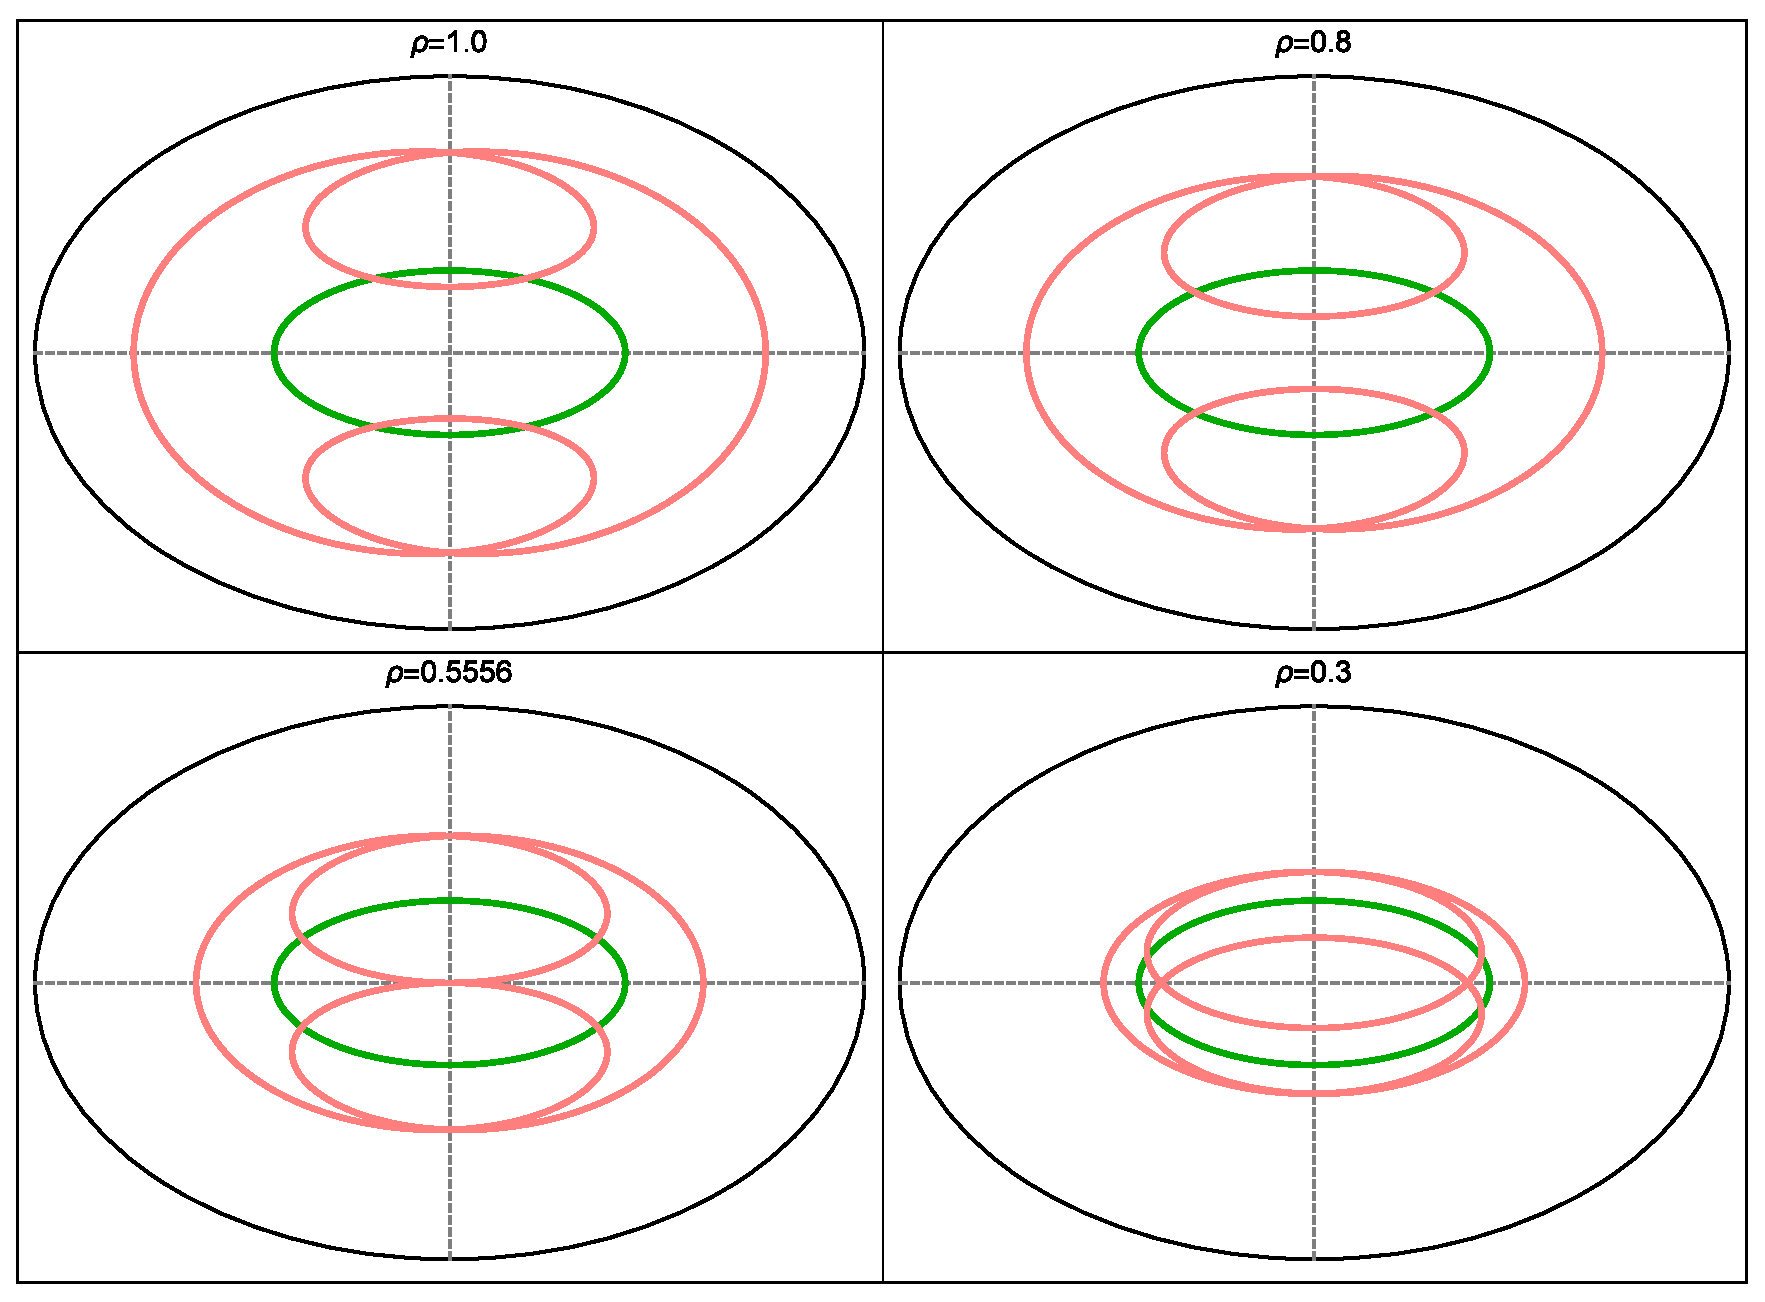
\includegraphics[width=\textwidth]{pics_05_110_conv_inc_pedal}
    \caption{The locus (pink) of a convex combination of an intouchpoint and the incenter for different values of $\rho$. When $\rho=0$ (top left), one obtains the original locus of an intouchpoints. When $\rho=1$ (bottom right), one obtains the elliptic locus of the incenter (green). \href{https://youtu.be/3Gr3Nh5-jHs}{Video 1}, \href{https://youtu.be/HZFjkWD_CnE}{Video 2}}
    \label{fig:05-inc-wind3}
\end{figure}
